\documentclass{egpubl}

% --- for  Annual CONFERENCE
% \ConferenceSubmission % uncomment for Conference submission
% \ConferencePaper      % uncomment for (final) Conference Paper
% \STAR                 % uncomment for STAR contribution
% \Tutorial             % uncomment for Tutorial contribution
% \ShortPresentation    % uncomment for (final) Short Conference Presentation
%
% --- for  CGF Journal
 \JournalSubmission    % uncomment for submission to Computer Graphics Forum
% \JournalPaper         % uncomment for final version of Journal Paper
%
% --- for  CGF Journal: special issue
% \SpecialIssueSubmission    % uncomment for submission to Computer Graphics Forum, special issue
% \SpecialIssuePaper         % uncomment for final version of Journal Paper, special issue
%
% --- for  EG Workshop Proceedings
% \WsSubmission    % uncomment for submission to EG Workshop
 %\WsPaper         % uncomment for final version of EG Workshop contribution
%
 \electronicVersion % can be used both for the printed and electronic version

% !! *please* don't change anything above
% !! unless you REALLY know what you are doing
% ------------------------------------------------------------------------

% for including postscript figures
% mind: package option 'draft' will replace PS figure by a filname within a frame
\ifpdf \usepackage[pdftex]{graphicx} \pdfcompresslevel=9
\else \usepackage[dvips]{graphicx} \fi

\PrintedOrElectronic

% prepare for electronic version of your document
\usepackage{t1enc,dfadobe}
\usepackage{url}
\usepackage{algorithm2e}
\usepackage{mathptmx}
\usepackage{graphicx}
\usepackage{times}
\usepackage[usenames,dvipsnames,svgnames]{xcolor}
\usepackage{subfigure}
\usepackage{flushend}
\usepackage[compact]{titlesec}
\usepackage[normalem]{ulem}

\usepackage{egweblnk}
\usepackage{cite}

%\usepackage[bookmarks,backref=true,linkcolor=black]{hyperref} %,colorlinks
%\hypersetup{
%  pdfauthor = {},
%  pdftitle = {},
%  pdfsubject = {},
%  pdfkeywords = {},
%  colorlinks=true,
%  linkcolor= black,
%  citecolor= black,
%  pageanchor=true,
%  urlcolor = black,
%  plainpages = false,
%  linktocpage
%}

% For backwards compatibility to old LaTeX type font selection.
% Uncomment if your document adheres to LaTeX2e recommendations.
\let\rm=\rmfamily    \let\sf=\sffamily    \let\tt=\ttfamily
\let\it=\itshape     \let\sl=\slshape     \let\sc=\scshape
\let\bf=\bfseries

\def\etal{\textit{et al.}}
\definecolor{MyGreen}{rgb}{0,0.7,0}
\definecolor{MyWhite}{rgb}{1,1,1}
\definecolor{MyGray}{rgb}{0.5,0.5,0.5}
\definecolor{LightGray}{rgb}{0.7,0.7,0.7}
\definecolor{DarkGray}{rgb}{0.3,0.3,0.3}
\definecolor{DarkYellow}{rgb}{0.7,0.7,0.0}
\definecolor{MyNavyBlue}{rgb}{0.2,0.3,0.7}
\definecolor{darkgreen}{rgb}{0,0.55,0}
\newcommand{\black}[1]{{\color{Black} #1}}
\newcommand{\white}[1]{{\color{MyWhite} #1}}
\newcommand{\gray}[1]{{\color{MyGray} #1}}
\newcommand{\red}[1]{{\color{red} #1}}
\newcommand{\green}[1]{{\color{MyGreen} #1}}
\newcommand{\blue}[1]{{\color{MyNavyBlue} #1}}
\newcommand{\yellow}[1]{{\color{DarkYellow} #1}}
\newcommand{\maybe}[1]{\yellow{#1}}
\newcommand{\rout}[1]{\red{\sout{#1}}}
\newcommand{\repl}[2]{\rout{#1} \green{#2}}
\newcommand{\fix}[1]{\red{\emph{(#1)}}}
\newcommand{\Fix}[1]{\begin{itemize} \renewcommand\labelitemi{\red{--}} \item \red{#1} 
\end{itemize}}

\newcommand{\todo}[1] {\textbf{[~}\textcolor {red}{#1}\marginpar{\textcolor {red}{\centerline{{\Huge \textbf{!}}}}}\textbf{~]}}
\newcommand{\question}[1] {\textbf{[~}\textcolor {darkgreen}{#1}\marginpar{\textcolor {darkgreen}{\centerline{{\Huge \textbf{!}}}}}\textbf{~]}}
\newcommand{\diff}[1]{[\textcolor{blue}{#1}\marginpar{\textcolor{blue}{\centerline{{\Huge \textbf{!}}}}}]}

\setlength\fboxsep{0pt}

% end of prologue

\title[Urban Search \& Rescue Mission Planning]{Supporting Urban Search \& Rescue Mission Planning\\ through Visualization-Based Analysis}

%\author{paper1006}
\author[Bock \etal]{
    Alexander Bock$^1$, Alexander Kleiner$^2$, Jonas Lundberg$^3$, and Timo Ropinski$^{1,4}$\\%
    $^1$ Scientific Visualization Group, Link\"oping University\\%
    $^2$ iRobot, Pasadena, CA\\%
    $^3$ Graphic Design Group, Link\"oping University\\%
    {\small $^4$ Visual Computing Group, Ulm University}
}   

%% Uncomment below to disable the manuscript note
%\renewcommand{\manuscriptnotetxt}{}

%% Copyright space is enabled by default as required by guidelines.
%% It is disabled by the 'review' option or via the following command:
% \nocopyrightspace

%%%%%%%%%%%%%%%%%%%%%%%%%%%%%%%%%%%%%%%%%%%%%%%%%%%%%%%%%%%%%%%%%%%%%%%%%%%%%%%%%%%%%%%%%%%
%%%%%%%%%%%%%%%%%%%%%%%%%%%%%%%%%%%%%%%%%%%%%%%%%%%%%%%%%%%%%%%%%%%%%%%%%%%%%%%%%%%%%%%%%%%

\begin{document}

\newcommand{\abTeaserImageHeight}{0.3\linewidth}
\teaser{
	\centering
	\subfigure[Voxelized 3D point cloud rendering that enables an increased awareness of an office building.]{
		\fbox{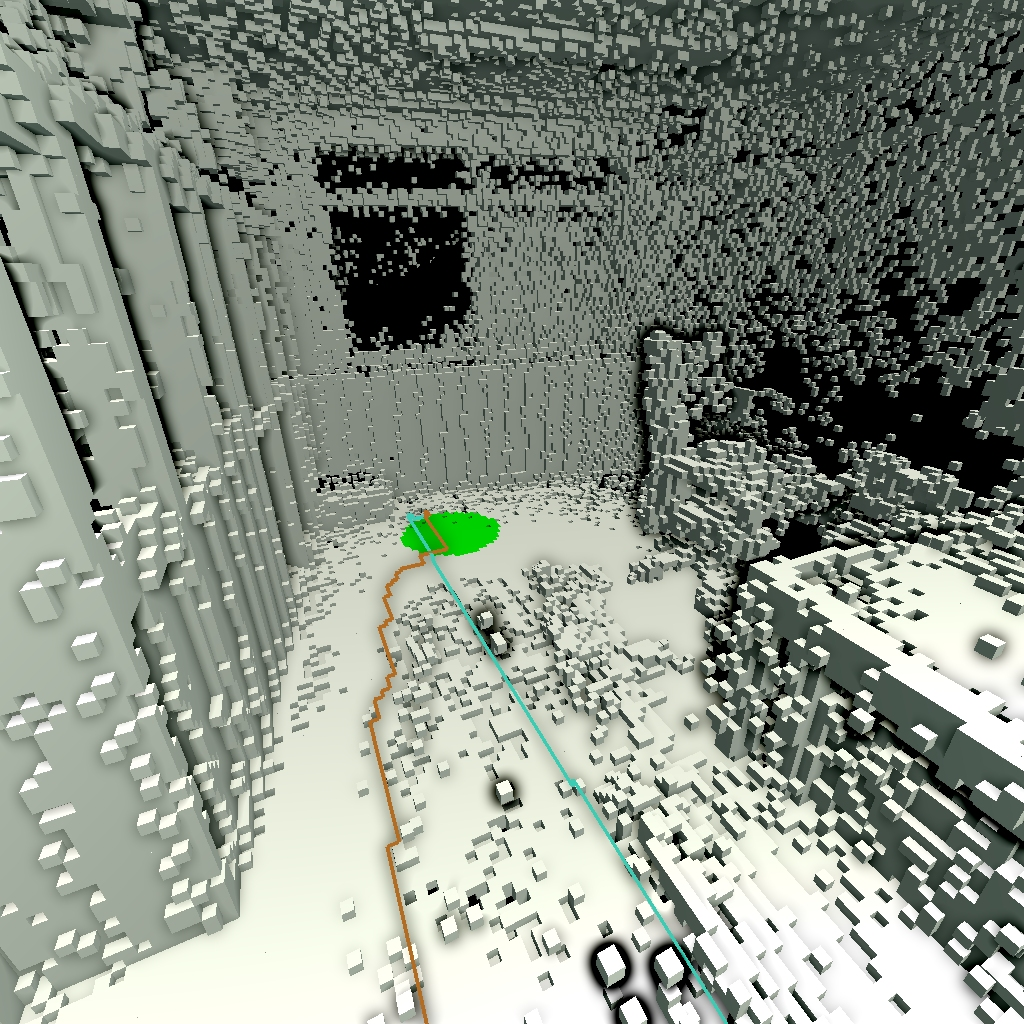
\includegraphics[height=\abTeaserImageHeight]{figures/image1.jpg}}\label{fig:teaser:1}
	}
	\hfill
	\subfigure[Viable paths through buildings of the Tohoku university with two hazardous environments.]{
		\fbox{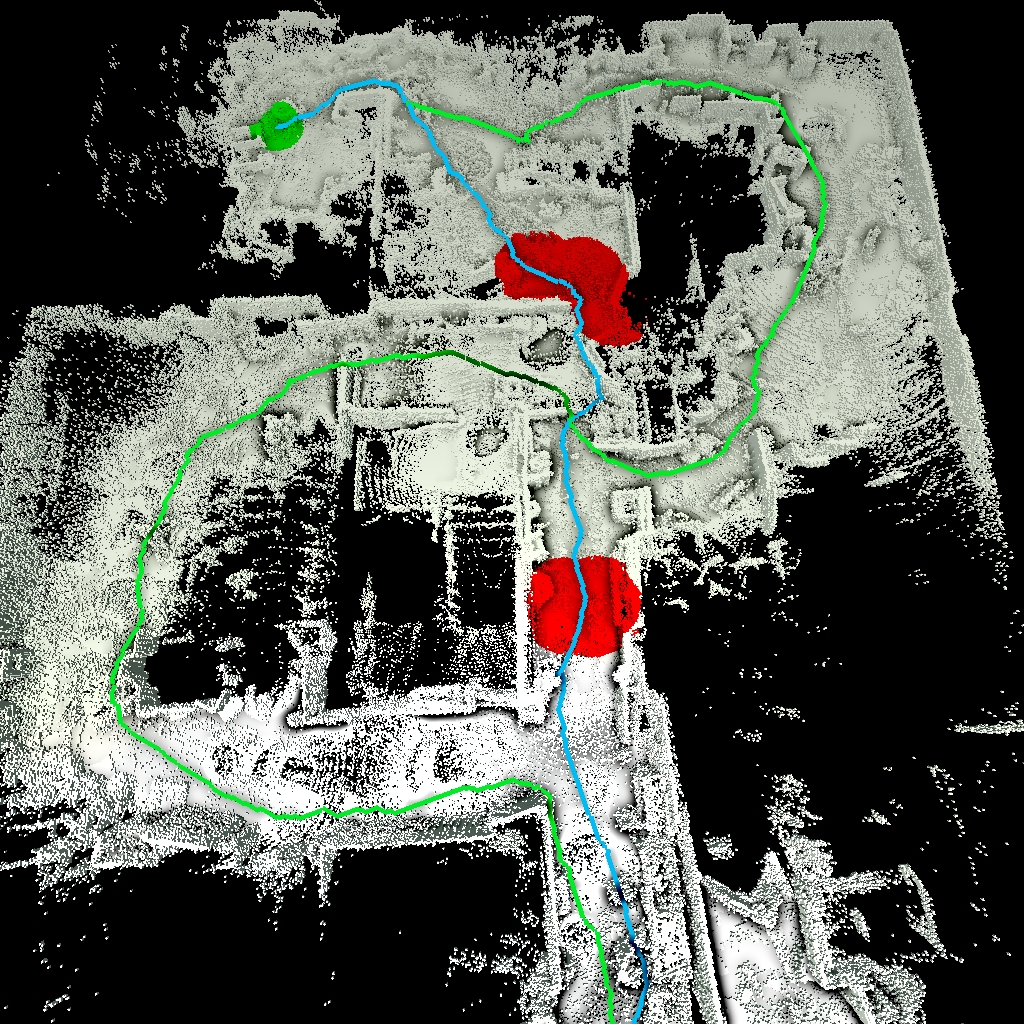
\includegraphics[height=\abTeaserImageHeight]{figures/image2.jpg}}\label{fig:teaser:2}
	}
	%\hfill
	%\subfigure[Top-down view of the area providing contextual information.]{
	%	\fbox{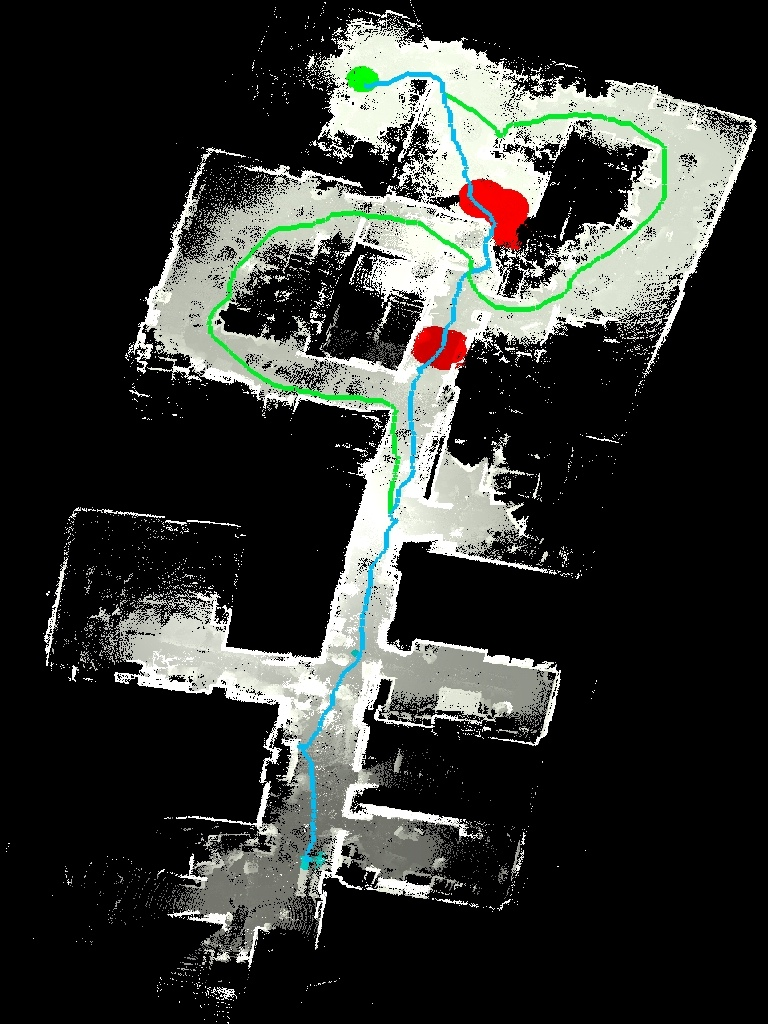
\includegraphics[height=0.2375\linewidth]{figures/image2-overview.jpg}}\label{fig:teaser:3}
	% }
	\hfill
	\subfigure[Path analysis using parallel coordinates plots and profile plots.]{
		\fbox{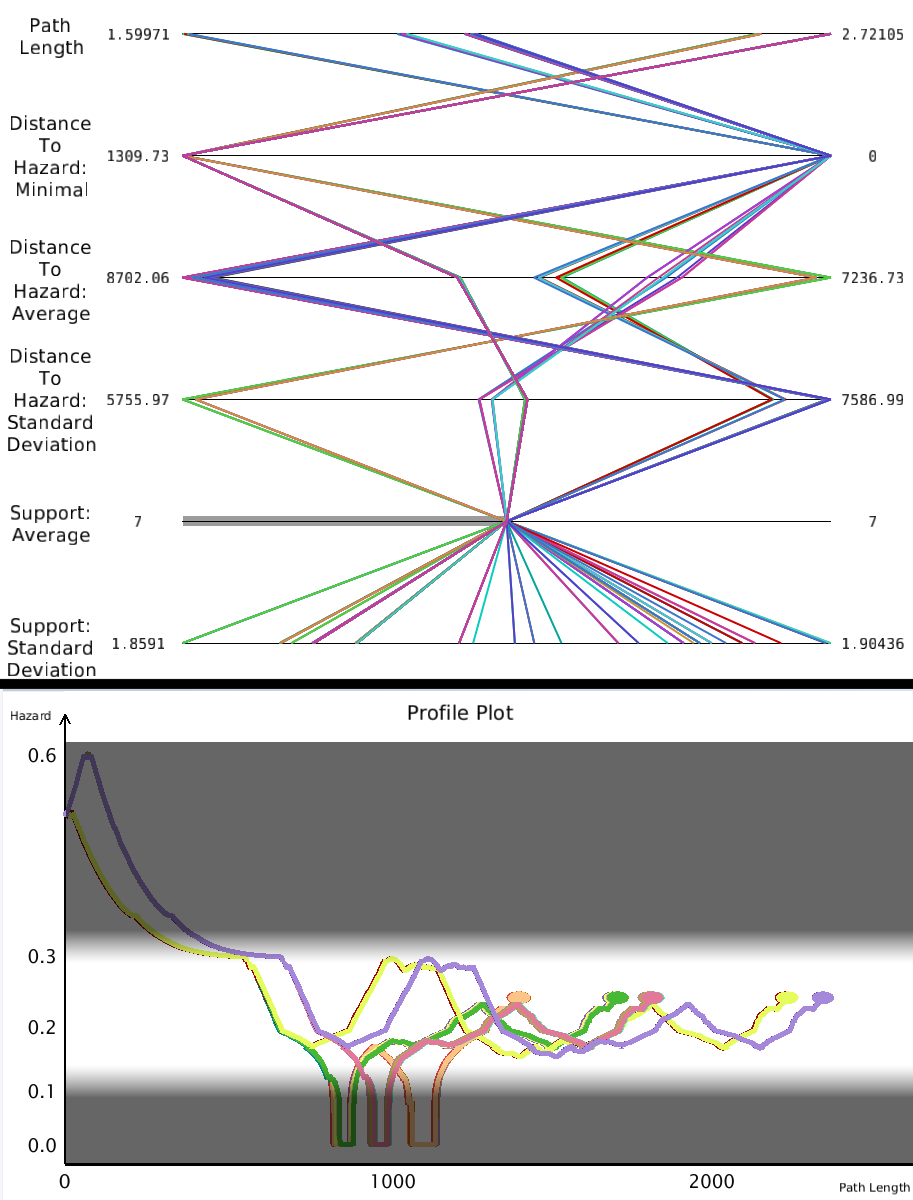
\includegraphics[height=\abTeaserImageHeight]{figures/pcpprofile.png}}\label{fig:teaser:4}
	}
  \caption{Our proposed visualization system applied to a collapsed building at Tohoku university. Different views (a,b) present the operator with an understanding of the building, allowing him to select and inspect paths that reach a point of interest. The assessment of the trade-off between paths is supported by a set of interactive visual analysis tools (c).}
  \label{fig:teaser}
}

\maketitle

\begin{abstract}
We propose a visualization system for incident commanders in urban search~\&~rescue scenarios that supports access path planning for post-disaster structures. Utilizing point cloud data acquired from unmanned robots, we provide methods for assessment of automatically generated paths. As data uncertainty and a priori unknown information make fully automated systems impractical, we present a set of viable access paths, based on varying risk factors, in an enhanced 3D environment combined with the visual analysis tools enabling informed decisions and trade-offs. Based on these decisions, a responder is guided along the path by the incident commander, who can interactively annotate and reevaluate the acquired point cloud to react to the changing dynamics of the situation. We describe design considerations for our system and decision support systems in general, technical realizations of the visualization components, and discuss the results of an expert evaluation.

\begin{classification}
   \CCScat{I.3.7}{Computer Graphics}{Three-Dimensional Graphics and Realism}{Color, shading, shadowing, and texture}
\end{classification}

\end{abstract}

\section{Introduction}
Structural damage to inhabited buildings is an ever-present danger. As time-to-rescue is an important factors for victims' survivability, it is of highest importance for rescue responders to reach victims and provide medical attention or extraction in a timely fashion. Planning and executing paths through buildings, however, is difficult as available floor plans are outdated. Furthermore, unknown structural weaknesses, as well as hazardous environments, make regions and areas of the building inaccessible. While trained responders use their knowledge and intuition to spot these hazards while traversing the structure, it is paramount that the \emph{Incident Commander} (IC) can analyze the information and coordinate multiple rescue responders simultaneously. There exist well-defined protocols describing the actions taken during an \emph{Urban Search~\&~Rescue} (USAR) operation. In most protocols, one IC is responsible for a single building and instructs multiple rescue responders inside. The Federal Emergency Management Agency, for example, describes distinct steps that are performed by the rescue team~\cite{fema08}. During the assessment step, two-dimensional maps of the collapsed building are hand-drawn based on the rescue responders' descriptions moving about the building in search for victims. During this exploration phase, they might stumble into hazardous areas that pose a threat to the rescuers' lifes.

In recent years, technological developments made it possible to use unmanned vehicles to perform this initial exploration step. The robots are equipped with sensors capable of detecting victims, gathering information about potentially hazardous environments, performing detailed scans of the interior layout, and streaming video data to the operator. This data is collated into a map, which the IC can use to plan access paths that reach certain \emph{Points of Interest} (POIs). In most cases, these POIs are potential locations of victims, but they can also be other mission critical areas.

In this paper, we propose a visualization system that creates an interactive 3D rendering tailored to increase the IC's awareness of internal structures (see Figure~\ref{fig:teaser}~(a,b)) and supports the planning and analysis of optimal access paths (see Figure~\ref{fig:teaser}~(c)). Our system computes an ensemble of access paths from an entry point to the POIs, in which each path is based on varying weighting factors. Uncertainty in the data and a priori unknown information make it infeasible to employ fully automatic algorithms to detect the globally optimal path. Instead, our system provides the IC with the tools to analyze and compare all available paths at once in order to make an informed trade-off. We describe system requirements, design considerations, technical realizations, and we discuss how experts perform in using the visualizations, how they rate their own understanding, and what preferences they have for the visualizations.

%%%%%%%%%%%%%%%%%%%%%%%%%%%%%%%%%%%%%%%%%%%%%%%%%%%%%%%%%%%%%%%%%%%%%%%%%%%%%%%%%%%%%%%%%%%
%%%%%%%%%%%%%%%%%%%%%%%%%%%%%%%%%%%%%%%%%%%%%%%%%%%%%%%%%%%%%%%%%%%%%%%%%%%%%%%%%%%%%%%%%%%

\section{Related Work} \label{sec:relatedwork}
\noindent {\bfseries Emergency management.} Much of the visualization-oriented work in the field of emergency management deals with evacuation planning before any disaster has occurred. Notable work was performed by Reddy~\etal, which enables analyzing possible bottlenecks of escape routes~\cite{EuroVA12:13-17:2012}. Ribarsky~\etal\ presented a system organizing first responders in intact structures~\cite{Ribarsky:2010}. Kim~\etal\ developed a system enhancing the situational awareness of responders using a mobile visual analytics tool~\cite{Kim:2008}. Many existing planning systems deployed nowadays in USAR scenarios are based on 2D representations~\cite{kleiner_et_al_ssrr09,KohlbrecherMeyerStrykKlingaufFlexibleSlamSystem2011}. Given the 2D map of the environment, one common approach to path planning is to plan the shortest trajectory and to follow this trajectory stepwise. Wirth~\etal\ introduced an exploration strategy and path planner that utilizes occupancy grid maps when planning to reach several targets at the same time~\cite{Wirth2007ETA1}.

\noindent {\bfseries Indoor navigation.}
   - Harris, M., The way through the flames, Spectrum, IEEE , vol.50, no.9, pp.30,35, September 2013
doi: 10.1109/MSPEC.2013.6587186
   - Fischer, Carl, and Hans Gellersen. Location and navigation support for emergency responders: A survey. IEEE Pervasive Computing 9.1 (2010): 38-47.
   - Wilson, J.; Bhargava, V.; Redfern, A; Wright, P., A Wireless Sensor Network and Incident Command Interface for Urban Firefighting, Mobile and Ubiquitous Systems: Networking & Services, 2007. MobiQuitous 2007. Fourth Annual International Conference on , vol., no., pp.1,7, 6-10 Aug. 2007

\noindent {\bfseries Point cloud visualization.} Basic rendering capabilities for point clouds are offered by the widely used Point Cloud Library~\cite{Rusu11ICRA}. There has been work by Richter~\etal\ using a level-of-detail structure to render massive point clouds at high frame rates~\cite{Richter:2010:ORV:1811158.1811178}. Xu~\etal\ showed that non-photorealistic rendering techniques can be applied to point cloud data~\cite{conf/npar/XuC04}. The contour lines in their rendering inspired our rendering algorithm. More recently, Pintus~\etal\ presented a rendering algorithm that enhances features of unstructured point clouds in real-time without preprocessing~\cite{Pintus:2011:RRM:2384495.2384513}. In our system, we use a voxelized point cloud representation that raises the level of abstraction and simultaneously provides an immersive experience for the IC in a similar fashion.

%%%%%%%%%%%%%%%%%%%%%%%%%%%%%%%%%%%%%%%%%%%%%%%%%%%%%%%%%%%%%%%%%%%%%%%%%%%%%%%%%%%%%%%%%%%
%%%%%%%%%%%%%%%%%%%%%%%%%%%%%%%%%%%%%%%%%%%%%%%%%%%%%%%%%%%%%%%%%%%%%%%%%%%%%%%%%%%%%%%%%%%

\section{Decision-Making Theory} \label{sec:theory}
It is crucial to take knowledge about human decision making into account when designing a decision support system. Andrienko and Andrienko showed that the usage of explorative interactive tools support the decision process~\cite{Andrienko:2003kv}. Decision makers tend to evaluate options serially in time-constrained situations; they attempt to find one viable plan rather than attempting to generate and compare numerous plans in parallel. This theory has been described by Klein and Calderwood as \emph{Recognition Primed Decision-making}~(RPD)~\cite{KleinCalderwood}. Initially, experts look for similarities to previous situations with a focus on relevant goals, things that were important to monitor, and possible actionable items. Then, they go through a process of mental simulation to consider whether these actions are applicable to the case at hand. They assess the ongoing situation, looking for violations and confirmations of expectations, which may require reframing the situation. Klein and Calderwood suggest that ``displays and interfaces should be centered on decisions rather than around data flows''~\cite{KleinCalderwood}, emphasizing that systems should be built to enhance the workflow of mental simulation. 

The \emph{Contextual Control Model}~(COCOM) by Hollnagel and Woods describes how people rely on context when making decisions~\cite{hollnagel2005joint}. Humans sometimes act with plans of lower quality, relying on the environment to make decisions opportunistically. The quality of their control can be described as scrambled, opportunistic, tactical, or strategic. The scrambled mode refers to decisions made without any information. In the opportunistic mode, people rely on cues in the local context to decide on their next action. In tactical mode, they have an idea how to achieve their goal before taking action---a plan. In strategic mode, the plan includes coordination with other simultaneous goals. Our aim is to raise the quality of control from being opportunistic (as in the current workflow) to being strategic, thus enabling improved decision-making capabilities.

The \emph{Extended Control Model}~(ECOM) describes plans in terms of a tactical level (setting goals), monitoring (making plans and overseeing plans), regulating (managing local resources), and tracking (performing and adjusting actions)~\cite{hollnagel2005joint}. This theory can be used to apprise what kind of planning support a system provides.  Moreover, it has been argued by Lundberg~\etal\ that it is important to support resiliency: ``Rather than merely selecting a response from a ready-made table, [the system] must adapt and create a suitable response; either by following ready-made plans for adaptation or by making sense of the situation and create responses during the unfolding event''~\cite{Lundberg2012}. Thus, in addition to supporting foreseeable responses, the system should also support working outside of prepared situations and be able to deal with changing circumstances.

%%%%%%%%%%%%%%%%%%%%%%%%%%%%%%%%%%%%%%%%%%%%%%%%%%%%%%%%%%%%%%%%%%%%%%%%%%%%%%%%%%%%%%%%%%%
%%%%%%%%%%%%%%%%%%%%%%%%%%%%%%%%%%%%%%%%%%%%%%%%%%%%%%%%%%%%%%%%%%%%%%%%%%%%%%%%%%%%%%%%%%%

\section{Incident Commander Workflow} \label{sec:workflow}

\begin{figure}
	\newcommand{\abWorkflowImageHeight}{\columnwidth}
	\centering
	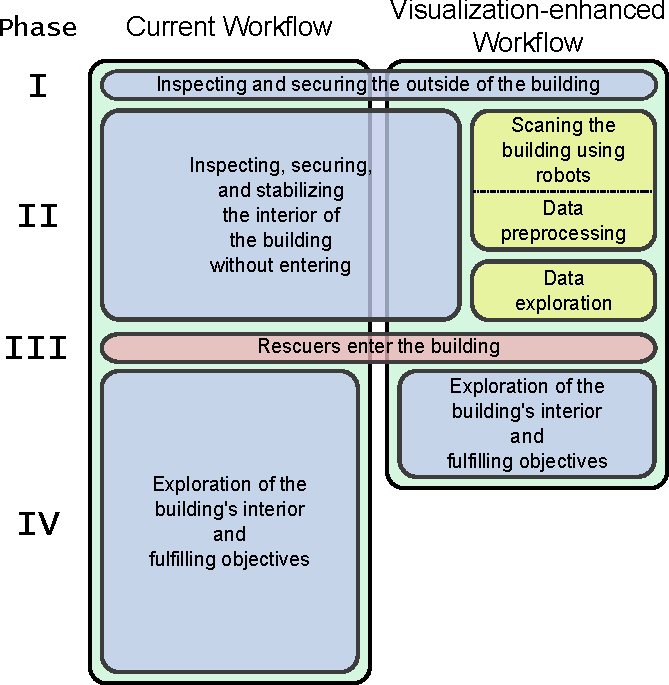
\includegraphics[height=\abWorkflowImageHeight]{figures/workflow.pdf}
	\caption{A schematic timeline overview of the currently employed workflow and our proposed system, showing events (red) and actions (blue) split up into four distinct phases. Utilizing additional actions (yellow) in parallel enables faster exploration and decreased overall time-to-rescue.}
	\label{fig:workflow:workflow}
\end{figure}

In this section, we will first describe the current workflow (see Figure~\ref{fig:workflow:workflow}, left) and then propose a visualization-enhanced workflow supported by our system (see Figure~\ref{fig:workflow:workflow}, right). The descriptions of the workflow is based on the information from the Federal Emergency Management Agency~\cite{fema08} and the Australian Emergency Management~\cite{em35}. Roman numerals in the text refer to the corresponding phases in the figure.

\noindent {\bfseries Current workflow.} The first step for the responders is to explore and secure the area outside the collapsed structure (Phase \texttt{I}). No rescuer is allowed to enter the building before it is secured, which can take multiple hours to finish (Phase \texttt{II}). Then, the IC determines viable entry points, rescuers enter the building and are directed by the IC to perform initial reconnaissance (Phase \texttt{III}). The rescuers inside the building slowly advance and report their progress to the IC, who draws a two-dimensional map of the interior based on their descriptions (Phase \texttt{IV}). The exploration of these unknown areas expose the rescuer to unknown risks, for example gas leaks or dormant fires. This is a good example of opportunistic control, where decisions are made opportunistically based on feedback from the environment and without global information. Although responders may recognize situations, decisions regarding the path are limited to the extent of the exploration and their view of the local environment. Global planning is further limited by the responders' ability to communicate relevant structural information accurately to the IC, such as angles of turns, which cause hand-drawn maps to experience drift.

\noindent {\bfseries Visualization-enhanced workflow.} The initial steps of securing the area are the same as in the currently employed workflow. While the responders are securing the building, the most time-consuming of the initial tasks, unmanned robots are released into the structure and perform the initial reconnaisance of the structure's inside, creating a three-dimensional map of the interior~(parallel execution in phase \texttt{II}). Furthermore, the robots' sensors are able to detect victims using thermal cameras and heart beat sensors~\cite{6027084, Wu12Eulerian}, but as these measurements are uncertain, false positives and false negatives might occur. The same holds true for hazardous environments like fires, gas leaks, structurally unsafe areas, chemical spills, radiation, or others. Data retrieval and preprocessing are done in parallel with securing the perimeter, so that all information is available when phase \texttt{III} begins. Based on suggested POIs, the system computes a set of optimal paths through the generated map, thus reducing time-to-rescue (Phase \texttt{IV}) as the rescuers do not need to explore the building to the same extent to find victims, but they can advance towards their location immediately. The proposed system applies RPD to the situation and extends the available planning from local conditions to higher ECOM levels as the IC and each rescue have information about the whole structure.

When planning the access paths, a variety of factors must be taken into account. The responder must maintain a safe distance from hazardous environments, avoid overhanging structures that might collapse with a rescuer beneath, and the ground must be stable and level. As these variables are extracted from the map, and are thus uncertain, they are subject to variability. The IC has to make trade-offs to choose between alternatives, for example favoring a longer, safer path over a shorter, more dangerous one.

While the IC is instructing the rescuer to follow one path, the rescuer feeds back information about victims or new hazards and the IC incorporates this information into the system. This is of high importance as features might not only have been missed by the robots, but detected features might change during the rescue operation. Fires can start or extinguish, subsequent collapses can make areas inaccessible, or additional passages are created after the initial reconnaissance by removing debris or breaching walls.

%%%%%%%%%%%%%%%%%%%%%%%%%%%%%%%%%%%%%%%%%%%%%%%%%%%%%%%%%%%%%%%%%%%%%%%%%%%%%%%%%%%%%%%%%%%
%%%%%%%%%%%%%%%%%%%%%%%%%%%%%%%%%%%%%%%%%%%%%%%%%%%%%%%%%%%%%%%%%%%%%%%%%%%%%%%%%%%%%%%%%%%

\section{System Overview} \label{sec:overview}

Combining expertise in visualization, cognitive systems engineering, rescue robotics, and informative discussions with rescue experts, we determined requirements to make our system useful for the IC. The visualization components are designed to comply with theories on sense-making and decision-making and have been tested in a user study with external domain experts. The requirements are as follows:
\begin{description}
\item[R1] The system must increase spatial awareness by allowing for interactive exploration of the collapsed structure.
\item[R2] The system must enable the IC to interactively annotate the acquired data to react to changing circumstances as desired by the ECOM.
\item[R3] The IC must be able to inspect all suggested access paths, compare them, and make viable trade-offs.
\item[R4] The system must provide the tools for the IC to select his chosen optimal path and support its execution.
\end{description}

The proposed system employs multiple linked views to address these requirements (see Figure~\ref{sec:overview:system}). In order to fulfill {\bfseries R1}, our system renders the point cloud at interactive frame rates while preserving occlusion information and thus helping the IC to form a consistent model of the collapsed structure. The IC can seamlessly annotate newly discovered entrances, hazards, POIs, and inaccessible areas directly in the rendering, thus fulfilling {\bfseries R2}. To address {\bfseries R3} and {\bfseries R4}, we integrate a visual representation of the different paths into the 3D visualization, and provide specific in-depth analysis tools.

The following sections address the components of our system. Before the acquired data can be used, a preprocessing must be performed (Section~\ref{sec:overview:preprocessing}). We describe the path computation process and the analysis together with comparison metrics in Section~\ref{sec:overview:pathcomputation}. Section~\ref{sec:overview:annotation} explains the annotation of the point cloud. Lastly, Section~\ref{sec:overview:3dvisualization} provides details on the considerations that went into designing the visualization components of our system.

\begin{figure}
	\newcommand{\abSystemScreenshotWidth}{\columnwidth}
    \centering
    \framebox[\columnwidth][c]{
        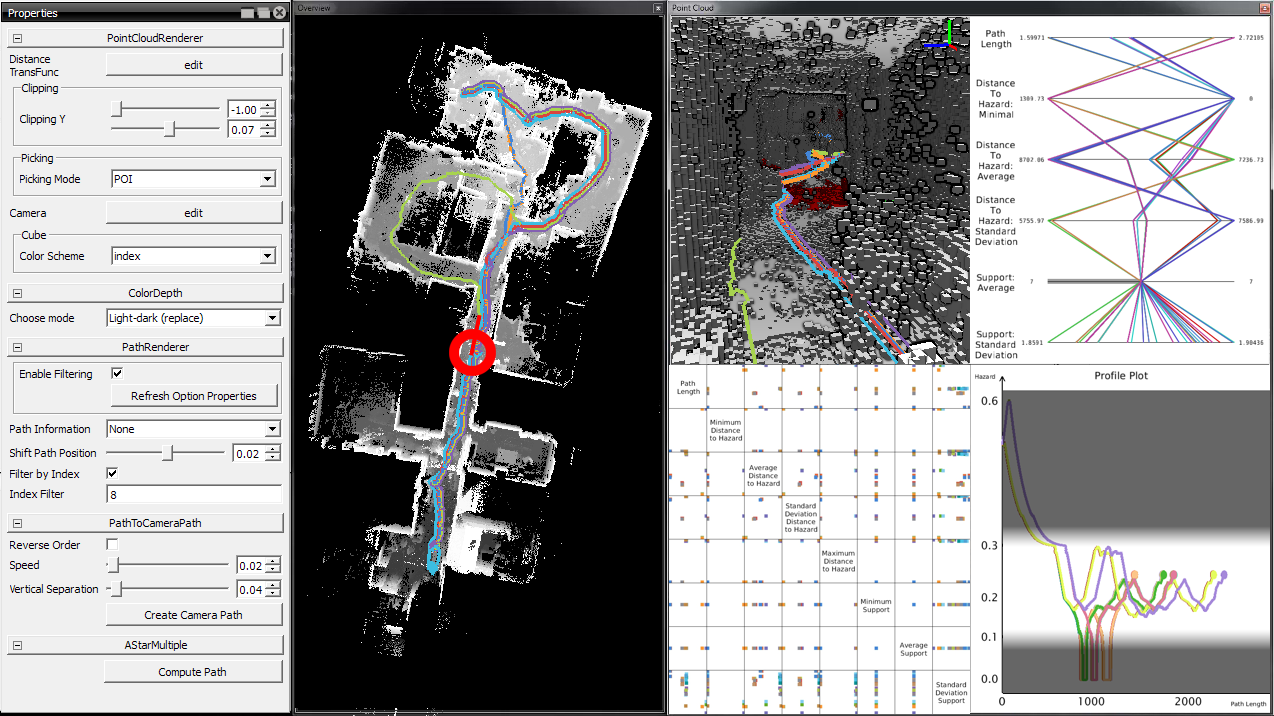
\includegraphics[width=\columnwidth]{figures/fig-overview-system2.png}
    }
    \caption{A screenshot of our system for a typical scenario. Settings on the left are global parameters and can be mapped to keyboard keys for easy access, the center view provides a bird's eye view onto the structure giving contextual information. The right view allows for detailed inspection of different paths and navigation in the three-dimensional environment. Each subview can be maximized.}
    \label{sec:overview:system}
\end{figure}


\subsection{Data Preprocessing} \label{sec:overview:preprocessing}
The retrieved data from the unmanned robots is an unstructured, annotated point cloud. One issue with rendering such point clouds is missing occlusion information and the non-uniform distribution of measured points. To avoid this problem, we perform a binning to obtain a three-dimensional voxel data structure on a regular grid. The voxel size is dependent on the scan resolution of the robot, and is a trade-off between resolving smaller details and increasingly noisy data. In our cases, voxel sizes of about 5\,cm were sufficient in all test cases with regard to this trade-off. From this point on we call a measurement in the original point cloud a \emph{point} and refer to a position in the grid-based, binned point cloud as a \emph{voxel}.

\noindent {\bfseries Attribute derivation.} In the second part, derived attributes are computed on the voxel grid that are later used to determine the set of rescue paths and to support and inform their analysis. Figure~\ref{fig:imageenhancement:colors} shows a selection of these attributes. We compute a \emph{hazard distance field} (Figure~\ref{fig:imageenhancement:colors}, left) that denotes the distance to the closest hazard points. The \emph{support field} (Figure~\ref{fig:imageenhancement:colors}, right) shows the available supporting area for each voxel. This value determines whether there is enough floor available for a responder to walk on. The \emph{occupancy field} (Figure~\ref{fig:imageenhancement:colors}, center) denotes the number of points each voxel is based on. A higher occupancy means that the voxel contains more points in the original point cloud data and thus provides a higher certainty. The \emph{size field} shows for each voxel if a rescuer can fit into the space above the voxel. In the default settings, we calculate two size values, one with the rescuer standing up, and a second while crouching. However, the system is designed to allow easy integration of different geometries, such as additional unmanned robots. In order to compute viable paths, we also need orientation information to be able to exclude paths that would be too steep for a rescuer. The steepness of surfaces is approximated by the least-squares fitted plane based on all the points in the original point cloud that are covered by a voxel. The normal of the resulting plane is used as the normal for the voxel.

\subsection{Data Annotation} \label{sec:overview:annotation}
Each voxel can belong to one of five classes. \emph{Unclassified} is the default type for all voxels. \emph{Start} voxels are accessible entry points. This means that paths can start from any of these points. \emph{POI} voxels are destination points for paths. These indicates that there is a potential victim or another mission-critical element at this location, which needs to be reached. \emph{Hazard} voxels have been declared as dangerous due to, for example, an ongoing fire or a gas leak. Each hazard area has a normalized severity denoting how dangerous it is. These three classes can either be marked by the initial reconnaissance of the robot or interactively by the IC. \emph{Forbidden} voxels can only be declared by the IC and are areas completely out of reach. These points are used when, for example, a corridor collapses after the point cloud acquisition and is not accessible anymore. The classification for each voxel is modified by interacting with the 3D rendering using the mouse and keyboard, thus fulfilling {\bfseries R2}. 

\subsection{Path Computation} \label{sec:overview:pathcomputation}
We employ the widely used A* algorithm for the path computations~\cite{4082128}. The algorithm works as follows: For the current voxel $x$, the estimated remaining distance to the target is calculated for all unvisited neighboring voxels $y_i$. This value is the accumulated cost to reach $x$, the cost to move from $x$ to $y_i$ given a metric $m$, and the estimated cost to reach the target from $y_i$ using a heuristic. The neighboring voxel with the lowest cost is chosen as the next candidate. For a comprehensive description of the algorithm we refer to the book by Russel and Norvig~\cite{AStar}.

When computing a path, the metric $m$ determines the cost of moving from one voxel to its neighbor and thus the optimal path. However, it is possible to compute several optimal paths by changing this metric. The metric that is used in our system is composed of several, weighted sub-metrics that are summed up to yield:

\begin{equation}
\begin{array}{r@{}l}
m = & \textrm{L}_2(\mathbf{p},\mathbf{q}) + w_h \cdot \textrm{hazard}(\mathbf{q}) + w_s \cdot \textrm{size}(\mathbf{q}) + \vspace*{0.1cm} \\
  & w_n \cdot \textrm{normal}(\mathbf{q},\varphi) + w_{sup} \cdot \textrm{support}(\mathbf{q},n)
\end{array}
\label{eqn:metric}
\end{equation}

\noindent where $w_h$, $w_s$, $w_n$, and $w_{sup}$ are the weights that are varied between different path computations. $\mathbf{p}$ is the current voxel and $\mathbf{q}$ is the next voxel under consideration, $\textrm{hazard}(\mathbf{q})$ returns the hazard severity, $\textrm{size}(\mathbf{q})$ is a binary function that determines if there is enough space above the voxel $\mathbf{q}$, $\textrm{normal}(\mathbf{q},\varphi)$ computes the surface normal and returns a response between the maximum allowed deviation $\varphi$ and the gravity vector, and $\mathrm{support}(\mathbf{q},n)$ is the number of supporting voxels, with $n$ being a threshold determining the number of voxels needed to consider $\mathbf{q}$ being supported.

\subsubsection{Adaptive Sampling}

\begin{figure}
	\newcommand{\abSamplingComparisonWidth}{\linewidth}
	\centering
	\subfigure[Regular Sampling] {
		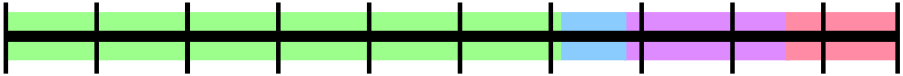
\includegraphics[width=\abSamplingComparisonWidth]{figures/regular_sampling.png}
		\label{fig:sampling:comparison:regular}
	}
	\subfigure[Adaptive Sampling using binary space partitioning] {
		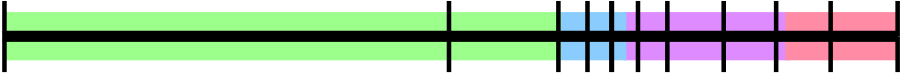
\includegraphics[width=\abSamplingComparisonWidth]{figures/adaptive_sampling.png}
		\label{fig:sampling:comparison:adaptive}
	}
	\caption{A comparsion between a regularly sampled one-dimensional parameter space and adaptive sampling. Vertical lines are samples, different colors symbolize different paths. In the regular sampling the green path is oversampled and the blue path is not sampled at all, while the adaptive sampling scheme samples all paths as evenly as possible.}
	\label{fig:sampling:comparsion}
\end{figure}

To generate path ensembles, the parameter space $P$ consisting of $w_h$, $w_s$, $w_n$, $w_{sup}$, $\varphi$, and $n$ has to be sampled. Each sample in $P$ is used to create a metric $m$ using Equation~\ref{eqn:metric}, which in turn is used by the A* algorithm to generate an optimal path. As there is no prior information about $P$ and no obvious correlation between samples and their resulting paths, providing a reasonable sampling strategy is not trivial. Using a regular grid to create samples is insufficient as it requires a priori information about reasonable boundary values, or else a large number samples will result in the same path, thus wasting computing effort (see Figure~\ref{fig:sampling:comparison:regular}). On the other hand, Markov Chain Monte Carlo methods~\cite{gilks2005markov} are also very sensitive to correct initialization, take a large amount of samples to converge, and are not trivial to parallelize. Instead, we implemented a sequential adaptive sampling technique based on binary space partitioning (see Figure~\ref{fig:sampling:comparison:adaptive}). Using the previously computed paths, new samples are only generated in regions that have the potential of yielding different paths. This rests on the intuitive assumption that if samples $p$ and $p \le q$ result in the same path $A$, all samples $p \leq r \leq q$ also yield $A$. The sampling algorithm is explained in Algorithm~\ref{alg:sampling} and illustrated for two-dimensional case in Figure~\ref{fig:sampling:adaptive}. All samples are separated into either non-recursive or recursive samples. In each iteration, every recursive sample will be tested against its neighboring samples to determine if a region should be subdivided. Please note that non-recursive samples do not occur in a one-dimensional parameter spaces, but are required in higher dimensions. For each iteration, each dimension is bisected and the resulting path for the bisecting sample is compared to the cornering paths. If the bisecting path is equal to a corner path, the recursion stops for that subspace. If they are different, a new bisector between the corner sample and the current bisector is created alongside necessary non-recursive samples. Figure~\ref{fig:sampling:adaptive} illustrates this step in two dimensions. The subdivision will continue until all recursive parameter values result in paths that have been computed before, thus not creating any new recursive samples, or until the distance between the samples is below a predefined $\epsilon$. This $\epsilon$ is necessary as the adaptivity would otherwise find the boundary between two paths and sampler closer to this boundary with each iteration.

\begin{algorithm}
Initialization\;
d $\leftarrow$ Number of dimensions\;
Creating $2^d$ non-recursive boundary samples\;
Creating one recursive sample value at 0.5\;
\While{new recursive samples exist}{
	\ForEach{$x$ in non-recursive samples}{
		compute path $p$ using the metric created from $x$\;
		update with path $p$\;
	}
	\ForEach{$x$ in recursive samples}{
		\If{distance $x$ to all corner values $< \epsilon$}{
			break\;
		}
		compute path $p$ using the metric created from $x$\;
		update with path $p$\;
		\ForEach{corner $c$}{
			\If{path of $c$ different is from $p$}{
				create $2^d$ non-recursive corner samples that have not been computed before or already exist in the non-recursive list\;
				create one recursive center sample by averaging all corner samples\;
			}
		}
	}
}
\caption{A pseudo-code overview of the implemented sequential adaptive sampling technique.}
\label{alg:sampling}
\end{algorithm}

\begin{figure*}
	\newcommand{\abSamplingImageWidth}{0.225\textwidth}
	\centering
	\subfigure[After the initialization step.]{
		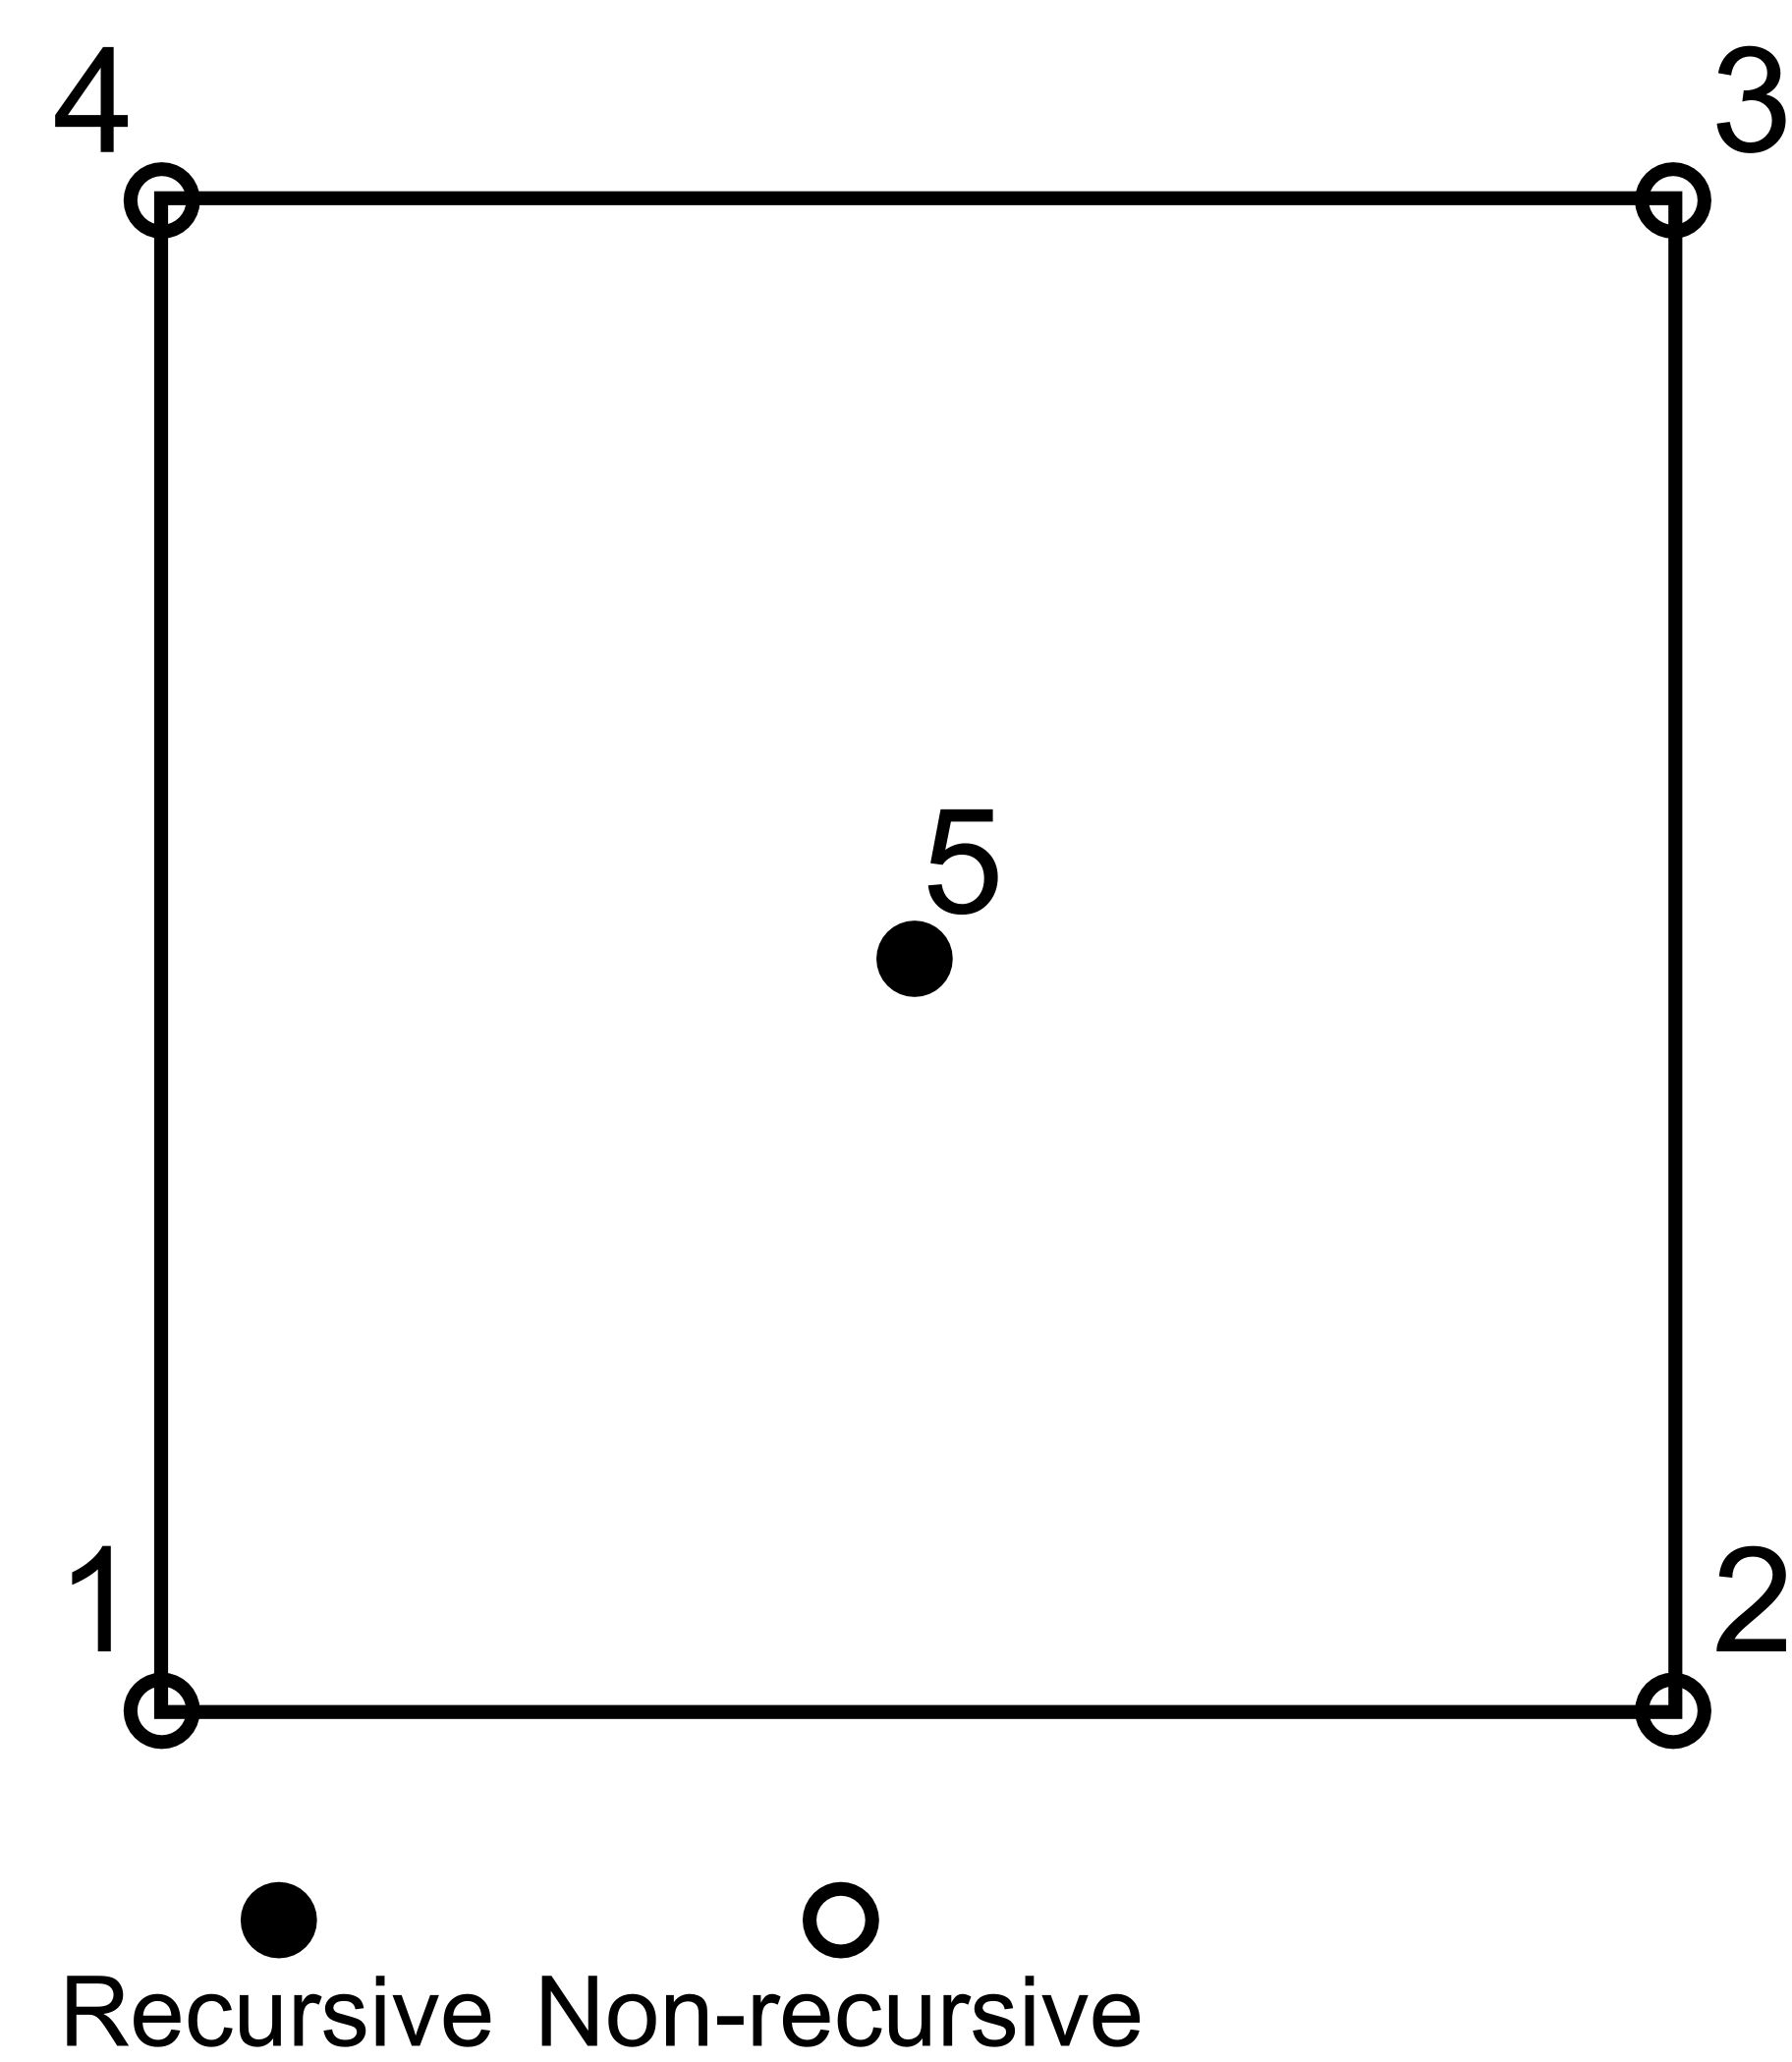
\includegraphics[width=\abSamplingImageWidth]{figures/adaptive_sampling_1.png}
		\label{fig:sampling:adaptive:1}
	}
	\hfill
	\subfigure[After the first iteration.]{
		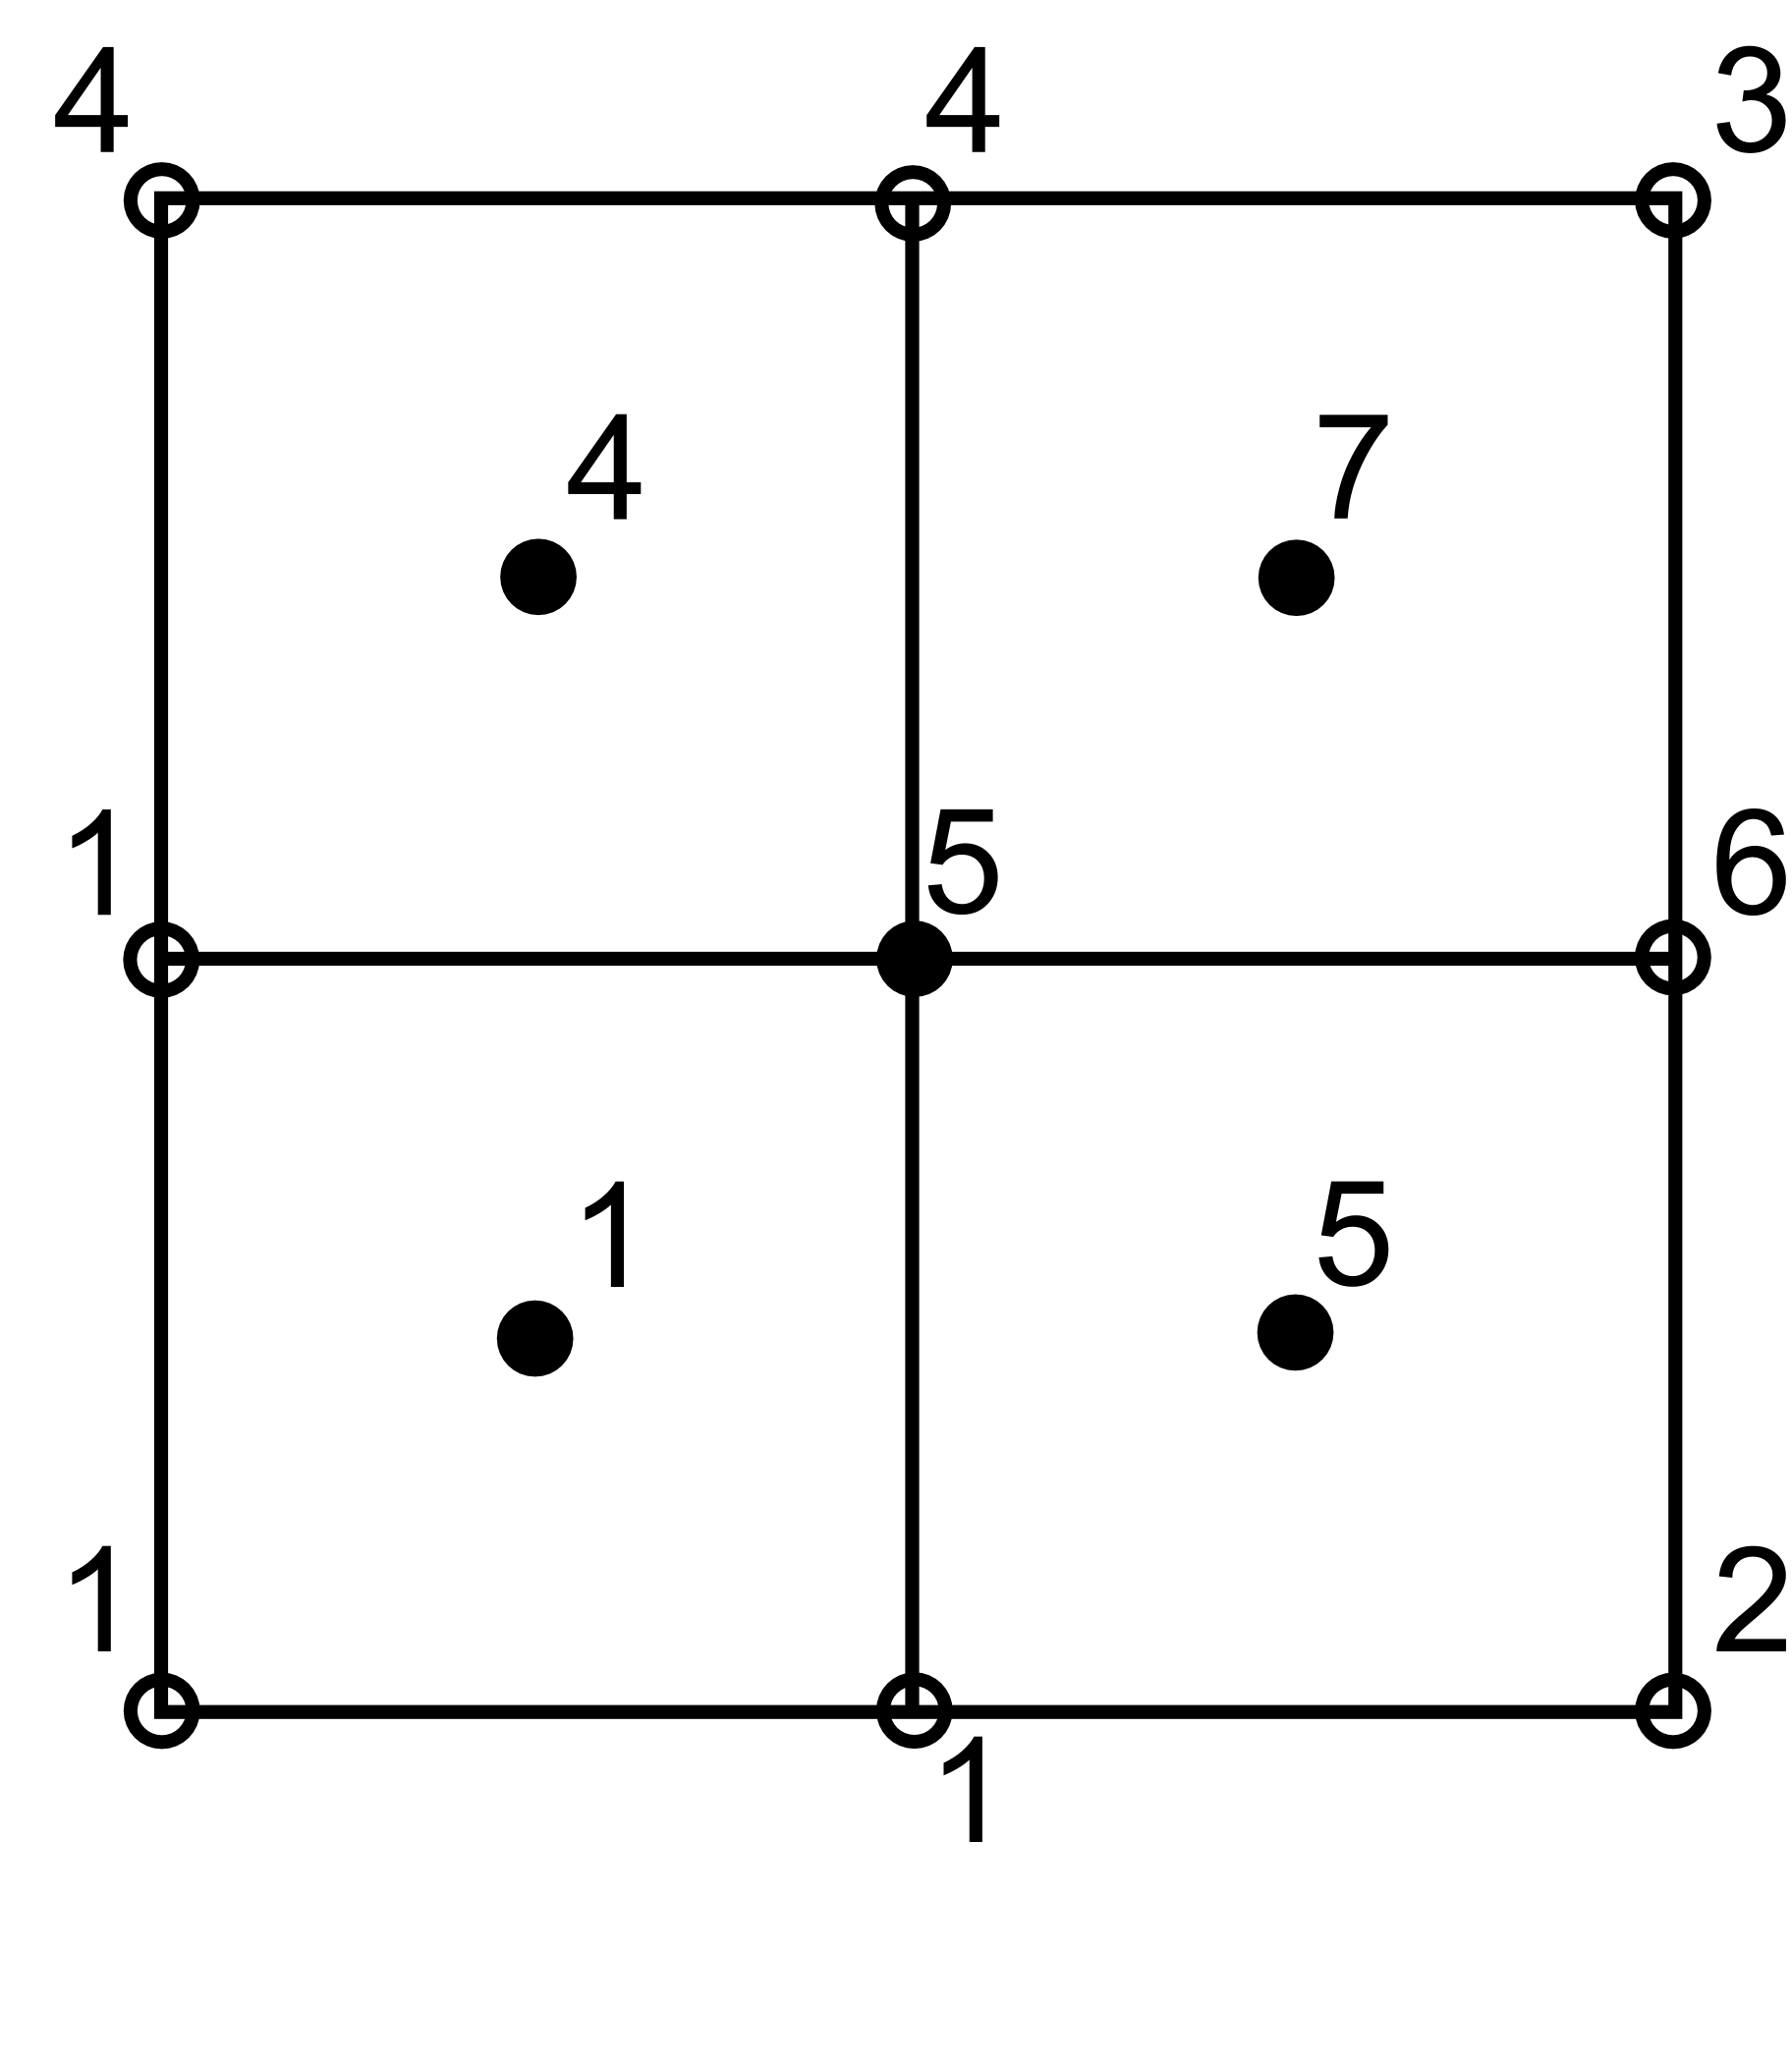
\includegraphics[width=\abSamplingImageWidth]{figures/adaptive_sampling_2.png}
		\label{fig:sampling:adaptive:2}
	}
	\hfill
		\subfigure[Showing regions that will not be subdivided during the second iteration.]{
		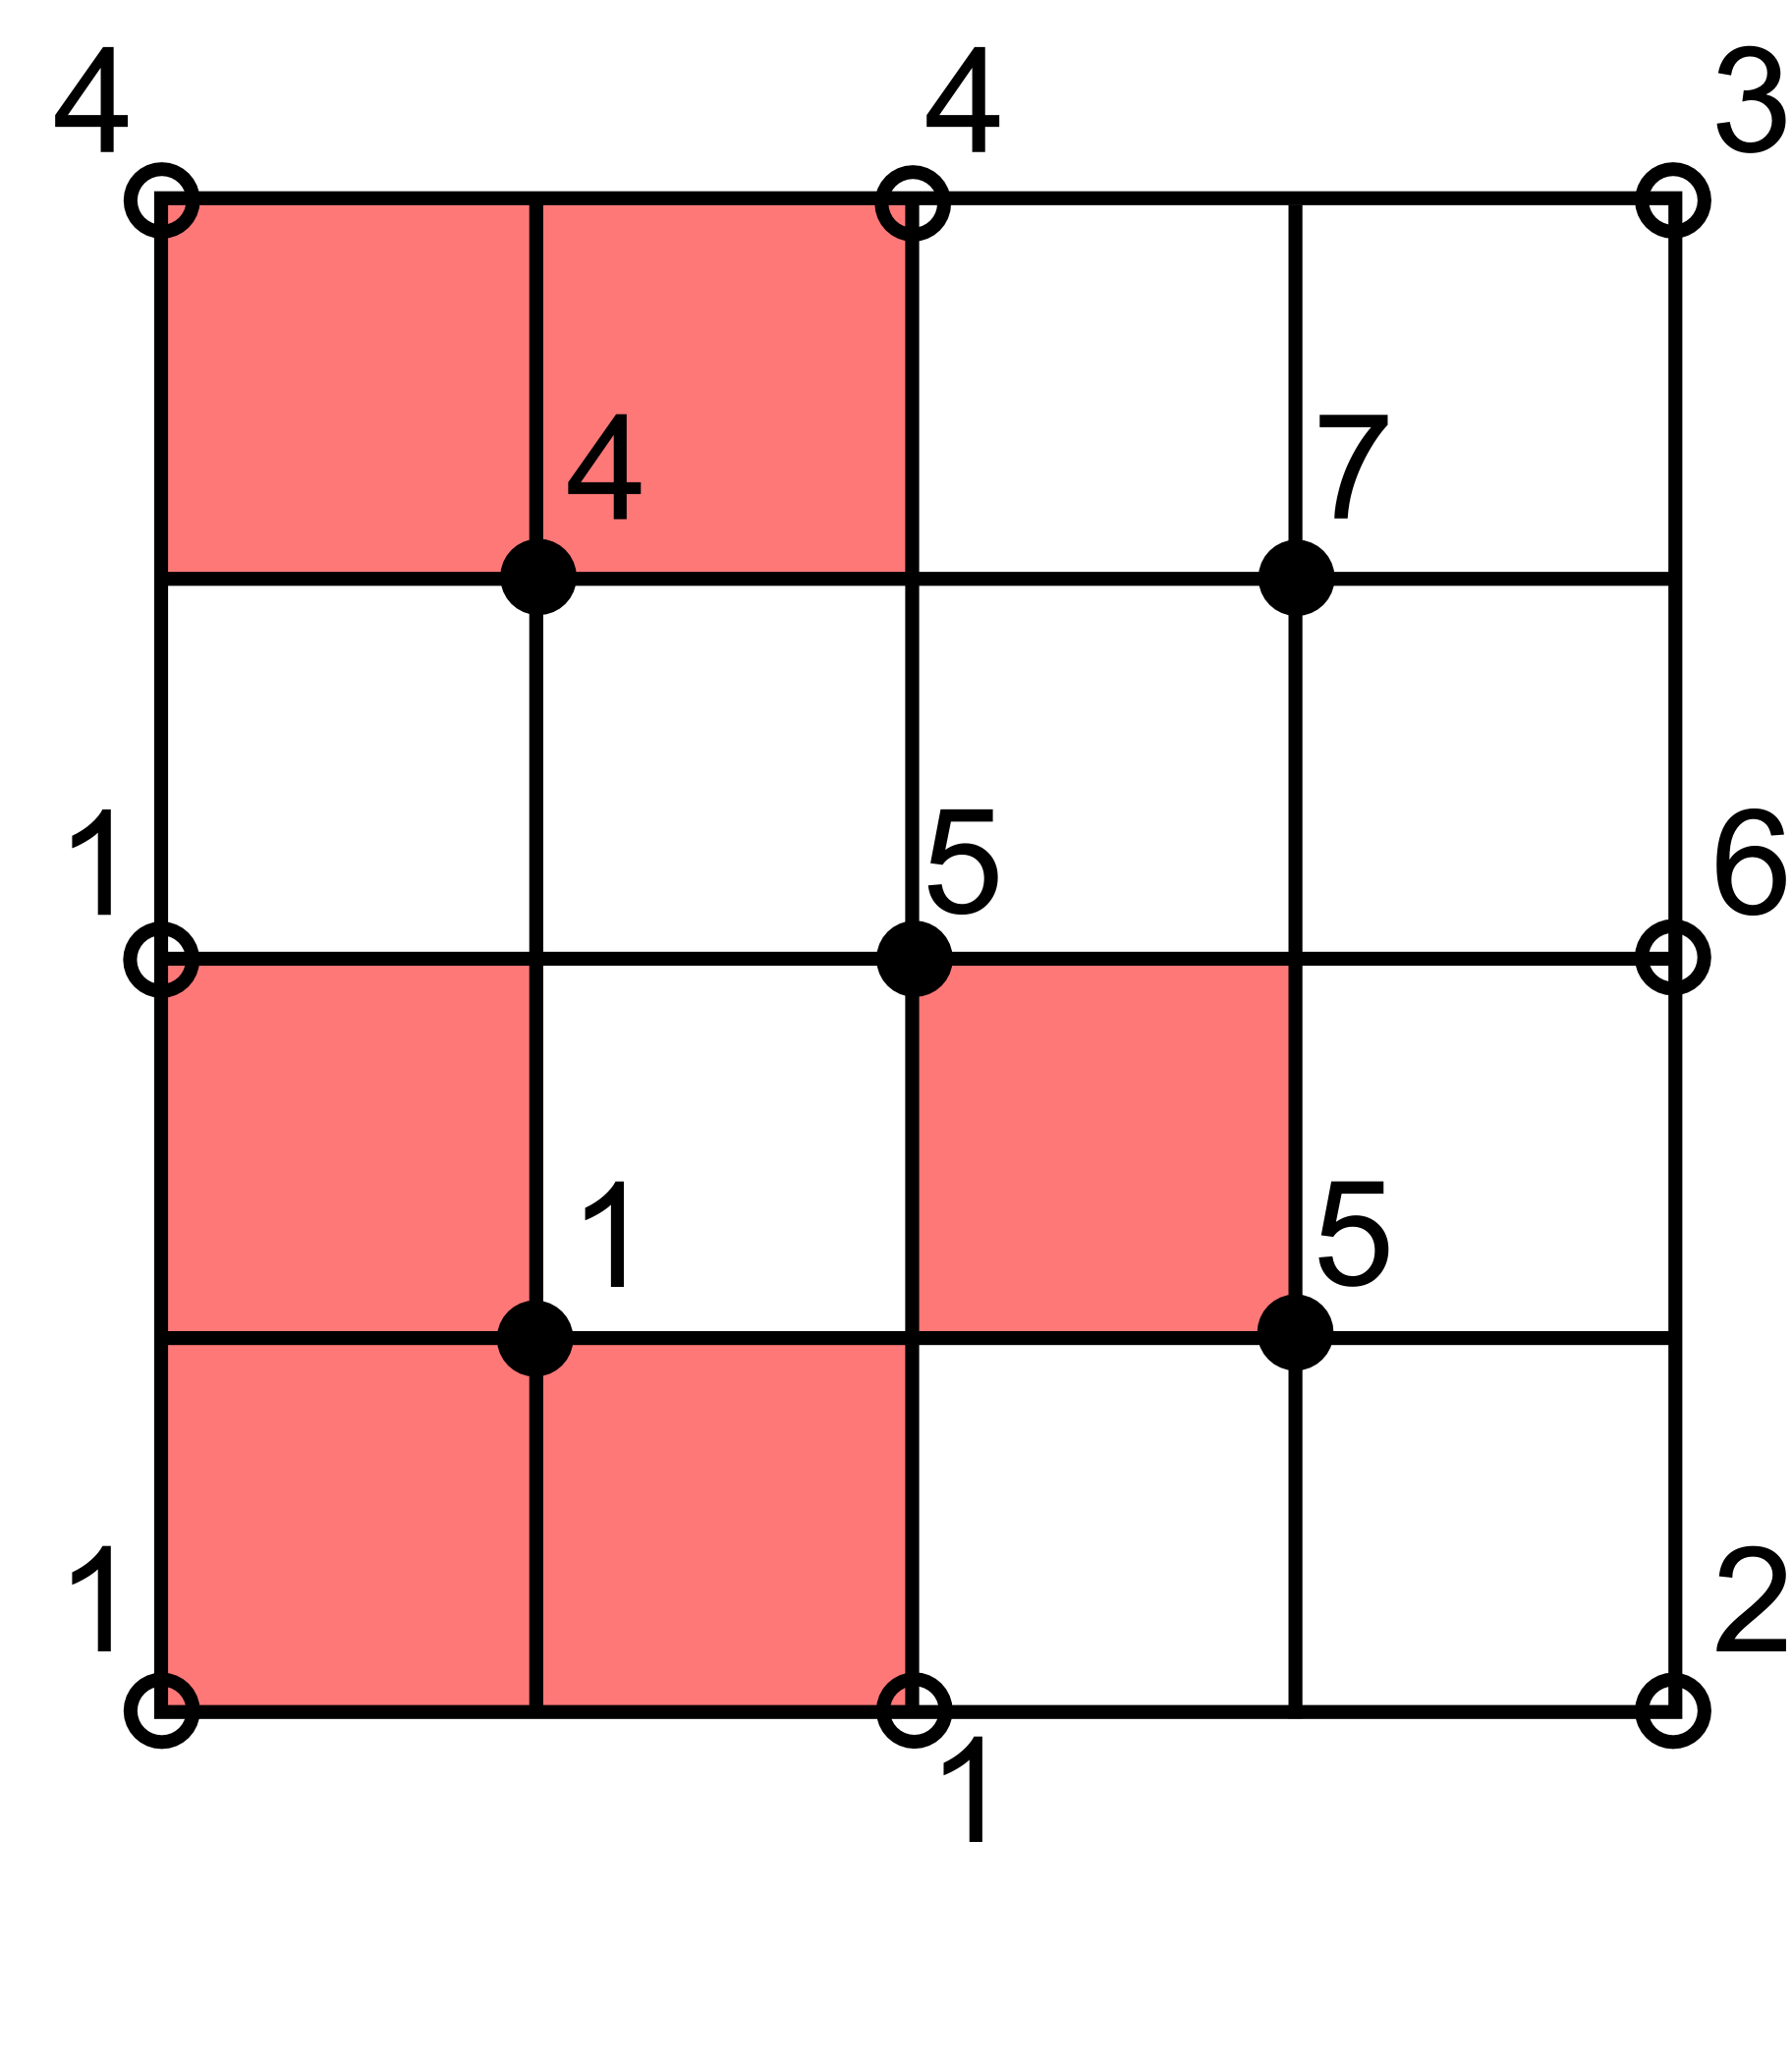
\includegraphics[width=\abSamplingImageWidth]{figures/adaptive_sampling_3.png}
		\label{fig:sampling:adaptive:3}
	}
	\hfill
		\subfigure[Including the samples generated in the second iteration.]{
		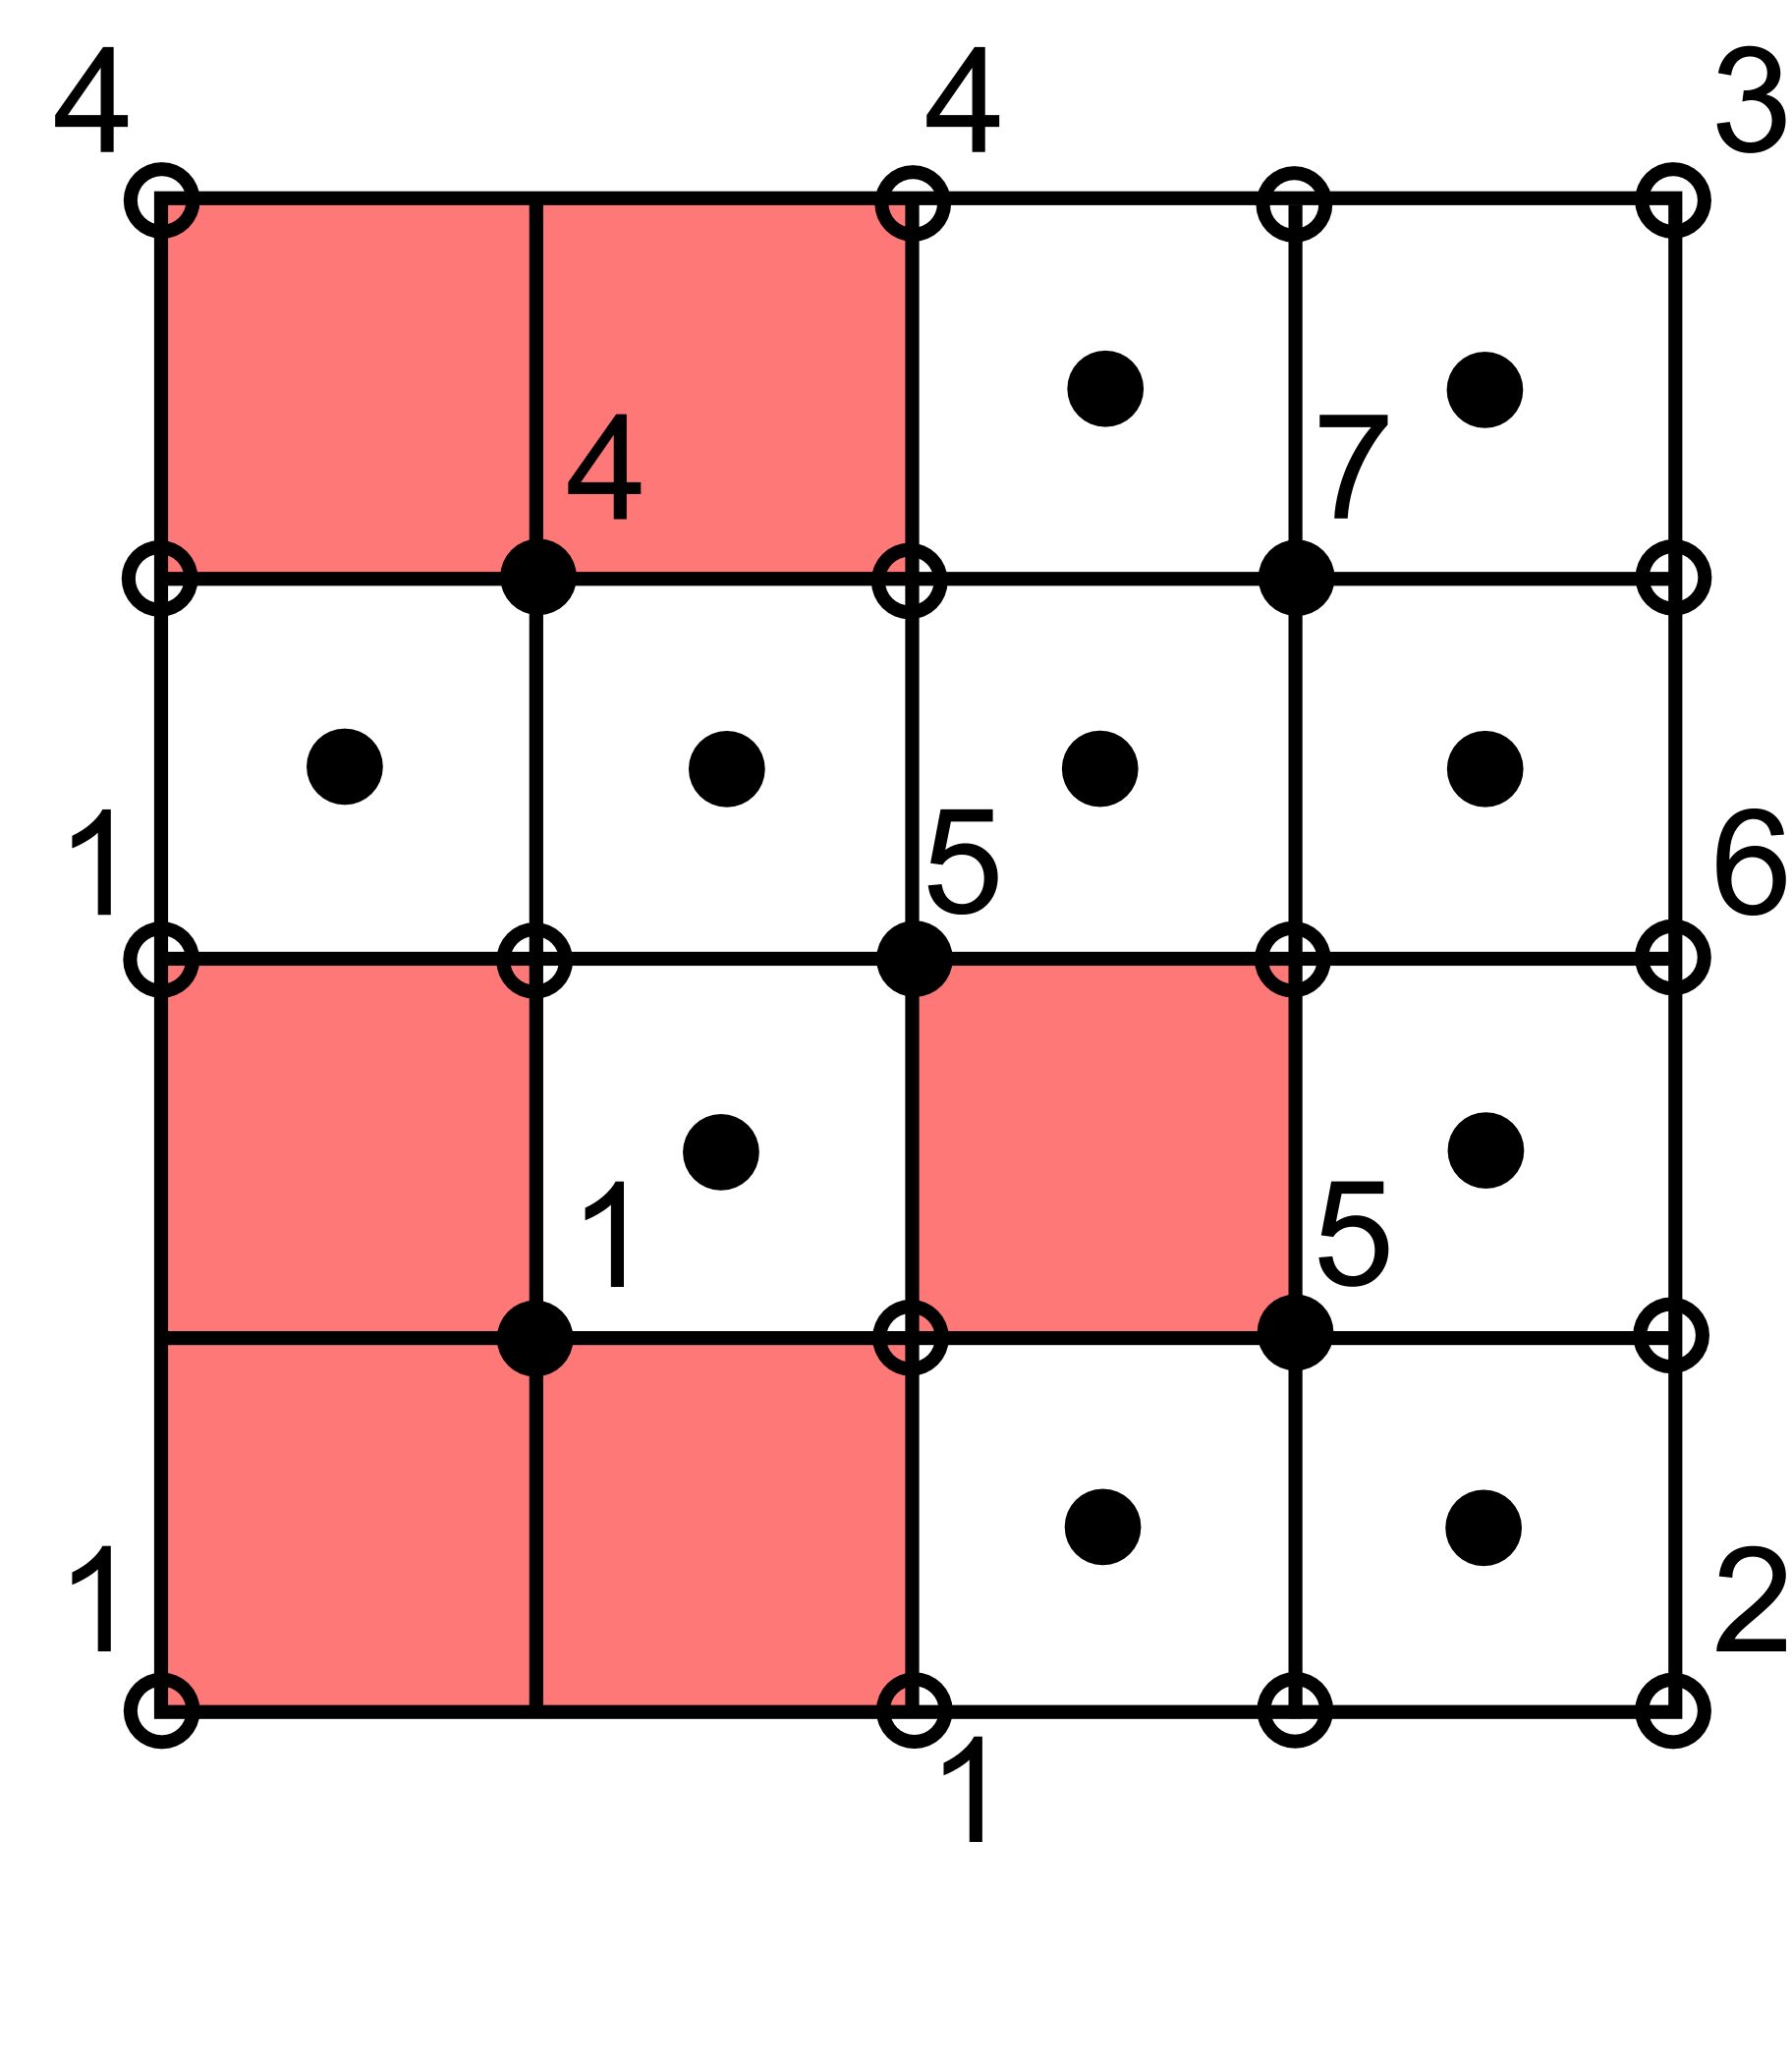
\includegraphics[width=\abSamplingImageWidth]{figures/adaptive_sampling_4.png}
		\label{fig:sampling:adaptive:4}
	}
	\hfill
	\caption{This figure illustrates the sequential adaptive sampling technique as described in Section~\ref{sec:overview:pathcomputation} using two dimensions. Full circles are recursive samples, outlined circles are non-recursive and numbers are identifiers for a path. After initialization, there is a non-recursive sample for each corner and a recursive sample in the center (a). In the first iteration, the central value is checked against each corner value and if they are different, new non-recursive samples as well as one recursive sample in the center are created (b). This process is performed recursively until there are no recursive samples left. Subfigure (c) shows the invalid areas during the second iteration, (d) shows the same iteration with the next samples inserted.}
	\label{fig:sampling:adaptive}
\end{figure*}

\subsection{Visual Path Analysis} \label{sec:overview:pathanalysis}
In our system, the IC uses linked views to filter the large number of computed paths in order to make informed decisions about an optimal trade-off. As the details of these trade-offs depend on the situation and the experience of the IC, we provide tools presenting information the IC requests, like \emph{Path Length} versus \emph{Minimal Hazard Distance} or \emph{Maximum Path Inclination} versus \emph{Minimal Support}. The employed views have been selected to support single and multiple path analysis, as well as the analysis of single and multiple attribute for each path. By using these views interactively, the IC can make full use of his knowledge in a strategic decision-making scenario. In the following, we will describe the intended role in the path analysis process for each view. As the path analysis begins with a large set of paths that needs to be filtered, views facilitating comparison of multiple global path attributes for several paths are used in the initial analysis phase. Later, the IC takes into account how attributes vary locally along the paths for a candidate subset of paths.

\subsubsection{Profile Plot} \label{sec:overview:analysis:profile}
In order to enable the analysis of attribute changes along a path, we include a \emph{Profile Plot} (PP). This variation of a line plot enables the IC to spot outliers among the paths and measurement errors that would present themselves as single spikes and shifts (see the violet line in Figure~\ref{fig:overview:analysis:profile}). It shows the distance travelled along the path on the x-axis and the IC can choose an attribute to inspect on the y-axis.

Several design considerations were made to ensure effective use of the PP. First, as a link between the 3D rendering and the other visualizations, the paths are shown in the same color as in the rendering with their end points being emphasized. Finally, the scale of the y-axis of the PP has been chosen such that attribute value discrimination becomes possible in regions of high importance. This is achieved by splitting the y-axis into a sub-linear, a linear, and a super-linear part. The separation occurs such that it provides a higher dynamic range to important values. An example of this remapping can be found in Figure~\ref{fig:overview:analysis:profile} that shows the \emph{Hazard Distance} on the y-axis. For this attribute, there is a non-linear importance of the value range, requiring higher detail for the important value differences. In addition, the IC can toggle a semi-transparent layer to further highlight the important value range. The transparency of the layer is proportional to the amount of remapping that was performed.

\subsubsection{Parallel Coordinates Plot} \label{sec:overview:analysis:pcp}
Figure~\ref{fig:overview:analysis:pcp} shows the \emph{Parallel Coordinates Plot} (PCP) of our system. PCPs are very well suited to detect patterns in the data, deviations from these patterns, and also to enhance interactive exploration of data sources~\cite{Tory05aparallel}.

In our system, the PCP axes show the derived global path attributes, for example \emph{Path Length}, \emph{Minimal Hazard Distance}, \emph{Average Hazard Distance}, or \emph{Standard Deviation of Support}. Through attribute exploration, the IC can move from a mental simulation of alternatives to simulation supported by the decision support system, thus amplifying RPD. The ability to explore trade-offs between alternative paths should facilitate a strategic COCOM decision mode for the targeting ECOM level. In addition to filtering of paths the IC can select a path in this view using the mouse and the interaction is replicated in the linked views. Furthermore, on request the IC can reorder the axis to suit his mental model interactively. Detecting previously unknown correlations and the ability to filter large parts of the data helps to fulfill {\bfseries R3} and {\bfseries R4}.

We have taken into account several design considerations for the PCP. One aspect is to avoid confusion introduced through the visual linking of the facilitated views. While using the same colors for same paths supports mental registration, we must ensure that this linking does not result in a direct mental matching of the different views. In the PP, the path length is mapped to the x-axis; this is not the case for the PCP, where the horizontal axis does not carry any spatial information. Therefore, we have chosen to avoid the horizontal layout usually adapted in PCPs and rotate the PCP by 90 degrees instead. A vertically oriented PCP is likely to be read from top to bottom, so the most important variables, \emph{Path Length} and \emph{Minimal Hazard Distance}, are displayed on the top of the plot. For an intuitive understanding of the path attributes, we have ordered each axis in such a way that preferable values are always on the left. 

Arranging the \emph{Minimal Hazard Distance} in the second row enables direct semantic grouping with the other hazard-related attributes. The support-related attributes indicate how comfortable it is for a human to take a path. To indicate that values below 50\,cm are not advisable, we gray out the value range between 0\,cm and 50\,cm. As the actually needed support depends on several parameters, we do not discard paths based on this parameter but instead apply this masking procedure to leave the final decision to the IC.

\subsubsection{Scatter Plot Matrix} \label{sec:overview:analysis:scatter}
The PCP is primarily used for aspects that we foresee that the IC wants to compare frequently. However, in line with the literature on resilience engineering~\cite{Lundberg2012} we also provide comparisons that cannot be foreseen in advance. Therefore, we use a Scatter Plot Matrix (SPLOM) to show relations between all attributes. Each individual scatter plot shows the correlation between two attributes and is used to verify known relationships or discover new correlations~\cite{Li2008}. Figure~\ref{fig:overview:analysis:scatter} shows the SPLOM.

\begin{figure*}
   \newcommand{\abInfoVisImageWidth}{0.3\textwidth}
	\centering
	\subfigure[Profile Plot]{
	    \fbox{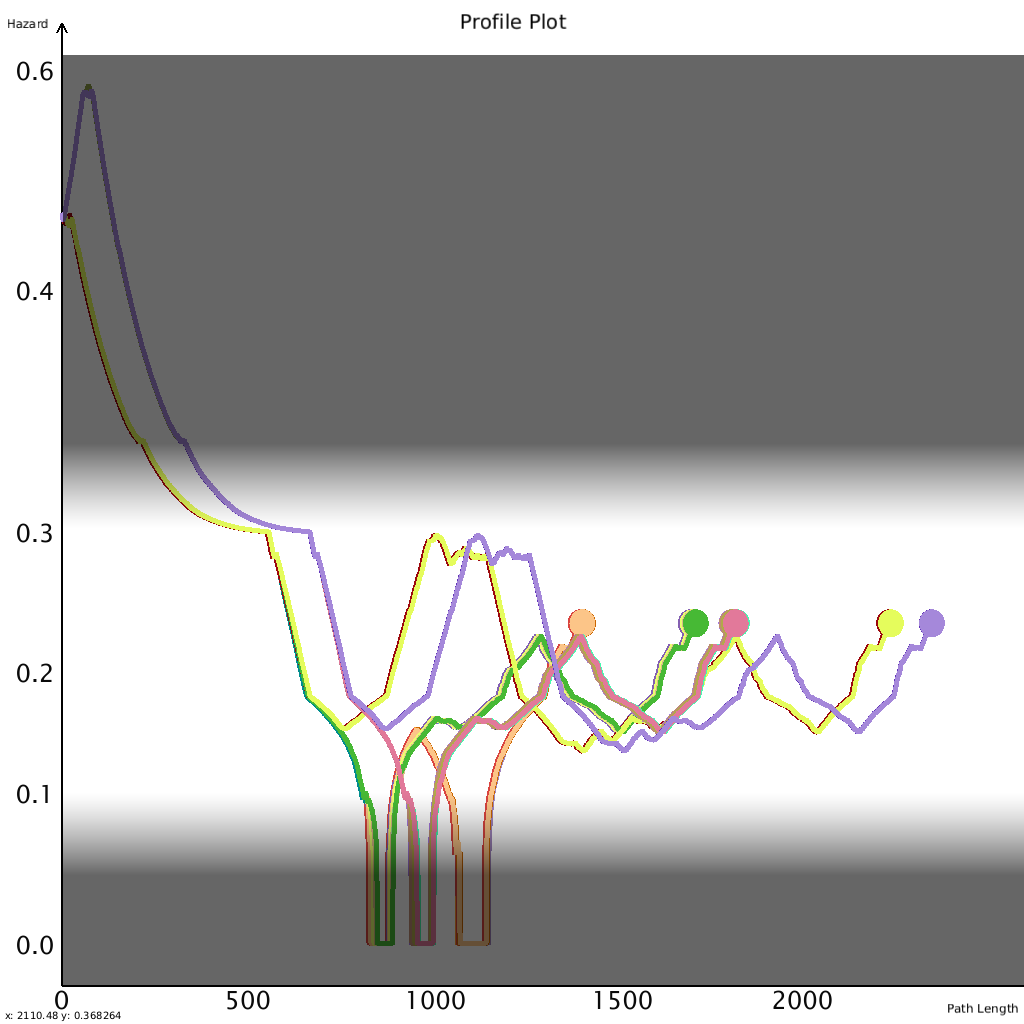
\includegraphics[width=\abInfoVisImageWidth]{figures/fig-analysis-profile.png}}
	    \label{fig:overview:analysis:profile}
	}
	\hfill
	\subfigure[Parallel Coordinates Plot]{
	    \fbox{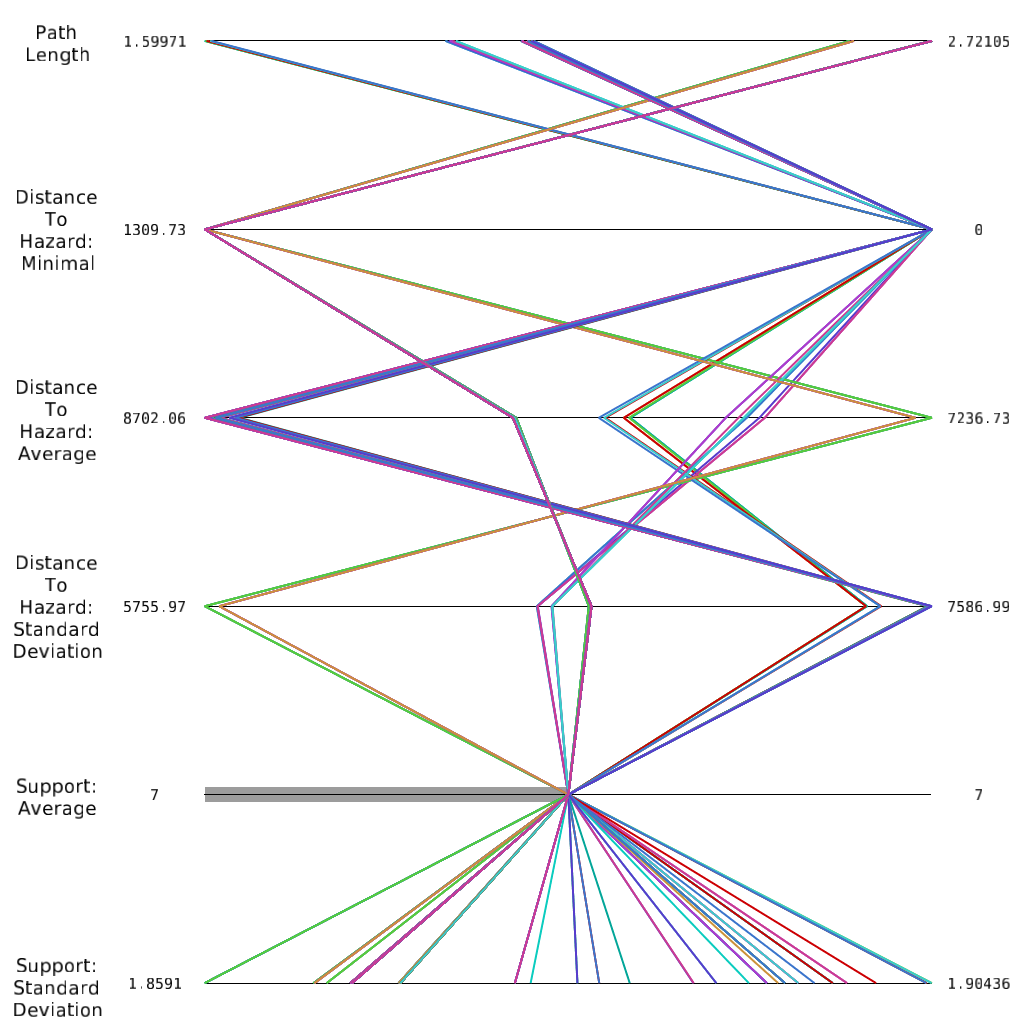
\includegraphics[width=\abInfoVisImageWidth]{figures/fig-analysis-pcp.png}}
	    \label{fig:overview:analysis:pcp}
	}
	\hfill
	\subfigure[Scatter Plot Matrix]{
	    \fbox{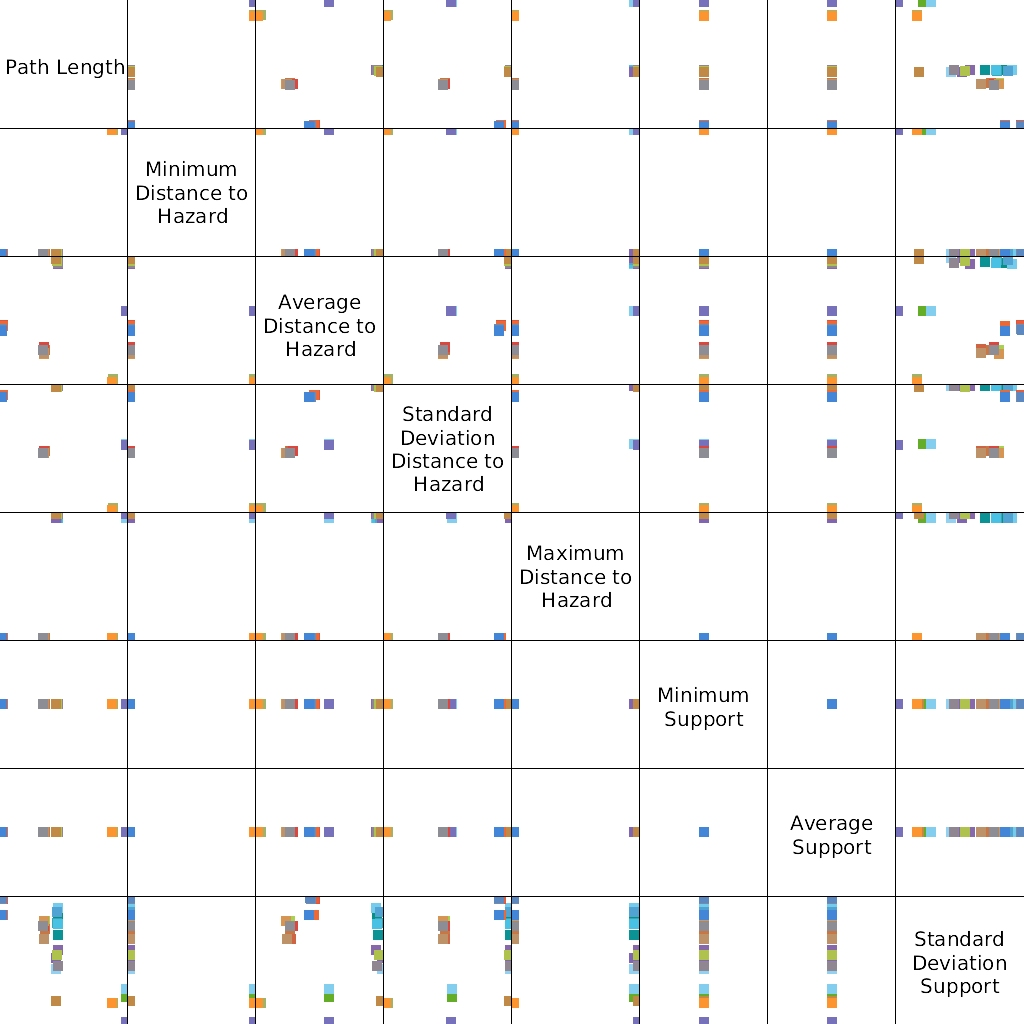
\includegraphics[width=\abInfoVisImageWidth]{figures/fig-analysis-scatter.jpg}}
	    \label{fig:overview:analysis:scatter}
	}
	\caption{Analysis views supporting the IC's comparative path analysis. The Profile Plot (a) presents the change of a single attribute over the length of each path; here the distance to the closest hazard. The Parallel Coordinates Plot (b) shows correlations between attributes. The Scatter Plot Matrix (c) depicts the correlations between all attributes.}
\end{figure*}

\subsection{3D Visualization} \label{sec:overview:3dvisualization}
\noindent {\bfseries Point cloud visualization.} Direct rendering of the unfiltered point cloud was insufficient, as missing depth cues inhibited the necessary immersion. A voxelized representation was chosen, as rendering each voxel using axis-aligned boxes solves the occlusion problem (Figure~\ref{fig:teaser}(a)). In addition to phong-shaded rendering, we provide a simulated depth image that maps the normalized depth to gray. This method resembles the output of range imaging cameras IC are already familiar with. In order to deal with structural occlusion, like a roof covering a building, the IC can interactively modify clip planes. Due to the discontinuous nature of the axis-aligned voxels, a camera-fixed setup of multiple light sources is used to provide suffient depth discrimination. The lights can be setup to not require any user interaction~\cite{wang2013lighting}.

\noindent {\bfseries Projective Texturing.} In order to provide the IC with access to image and recordings from robots that give him more detailed information on particular locations in the building, we implemented projective texturing~\cite{everitt2001projective}. Provided an orientation and a position, information that is readily available in the autonomous robots as they require this information for internal navigation, the acquired images or videos are projected onto the axis-aligned bounding boxes~\cite{1453517}. As this information will not be required at all times, the IC can enable and disable individual projected images interactively. Figure~\ref{fig:texturing} shows the Bremen Rescue arena~\cite{varsadan08} with two images taken by handheld cameras projected into the scene. As no location or orientation was available for these images, they have been positioned manually.

\noindent {\bfseries Bump Mapping.}  While it is possible for the IC to inspect the occupancy field mapped to color as in Figure~\ref{fig:imageenhancement:colors}, we found that in most situation the color information needs to be used for the detection of hazardous environments and thus cannot be used to show the occupancy field. In order to provide access to the hazard field and the occupancy field simultaneously, we implemented a bump mapping method that modifies up and down pointing normals based on a provided normal texture pattern. The texture is a structured noise pattern with periodic bounding conditions to inhibit artifacts between voxels. The strength of the bump mapping displacement is a linear dependence on the occupancy field. Due to the fact that the occupancy field consists mostly of radial patterns with decreasing occupancy towards the outside, this leads to an effect of the bump mapping fading out. This is preferable as sudden changes in the bump mapping would case too much attention to the features. This technique provides the IC with additional information about the reliability of each voxel without the need to switch between color maps, which would require a context switch for the IC. Figure~\ref{fig:imageenhancement:occupancy} shows the bump mapping on a floor at Tohoku University with the colored occupancy as comparison.

%\begin{figure}
%	\newcommand{\abBumpMappingImageWidth}{0.75\linewidth}
%	\centering
%	\subfigure[Bump Mapping] {
%		\fbox{\includegraphics[width=\abBumpMappingImageWidth]{figures/occupancy_bumpmapping.png}}
%		\label{fig:bumpmapping:bumpmapping}
%	}
%	\hfill
%	\subfigure[Color-Coded] {
%		\fbox{\includegraphics[width=\abBumpMappingImageWidth]{figures/occupancy_color.png}}
%		\label{fig:bumpmapping:color}
%	}
%	\caption{Comparison images of showing the voxels' occupancy using a bump mapping technique (a) and by coloring the voxels (b).}
%	\label{fig:bumpmapping}
%\end{figure}

\noindent {\bfseries Access path visualization.} In addition to using the same color as the other visualizations for each path, the IC can select a different coloring scheme to inspect the stored attributes of the paths. Each path attribute can be mapped to the path segments for a quick visual analysis. We enable the IC to select paths in the rendering, highlighting these paths in the linked views and desaturating all other paths.

The IC can use the visualization for a virtual walk-through to inspect whether a plan might actually work. It can be steered by the IC directly, or the camera can follows a selected path automatically. By inspecting this information, the IC can use his own experience to judge whether a path is feasible.

\noindent {\bfseries Immersive Environments.} In addition to the rendering capabilities of monitors, we provide the IC with the option of a more immersive rendering environment in which to inspect the data. We used this option to show a stereoscopic movie of the Tohoku application case and the rescue arena data set to an audience of approximately 100 researchers at an international conference on rescue robotics (see Figure~\ref{fig:immersive:fisheye}). We received positive informal feedback from these research experts on the rendering over the course of later discussions. Furthermore, this technique also allows the IC to inspect the rendering using a head-mounted display, such as the Oculus Rift (see Figure~\ref{fig:immersive:hmd}), which increases the users performance in search tasks~\cite{pausch1997quantifying}. 

\begin{figure*}
	\newcommand{\abImmersiveImageHeight}{0.25\linewidth}
	\centering
	\subfigure[Fisheye rendering] {
		\fbox{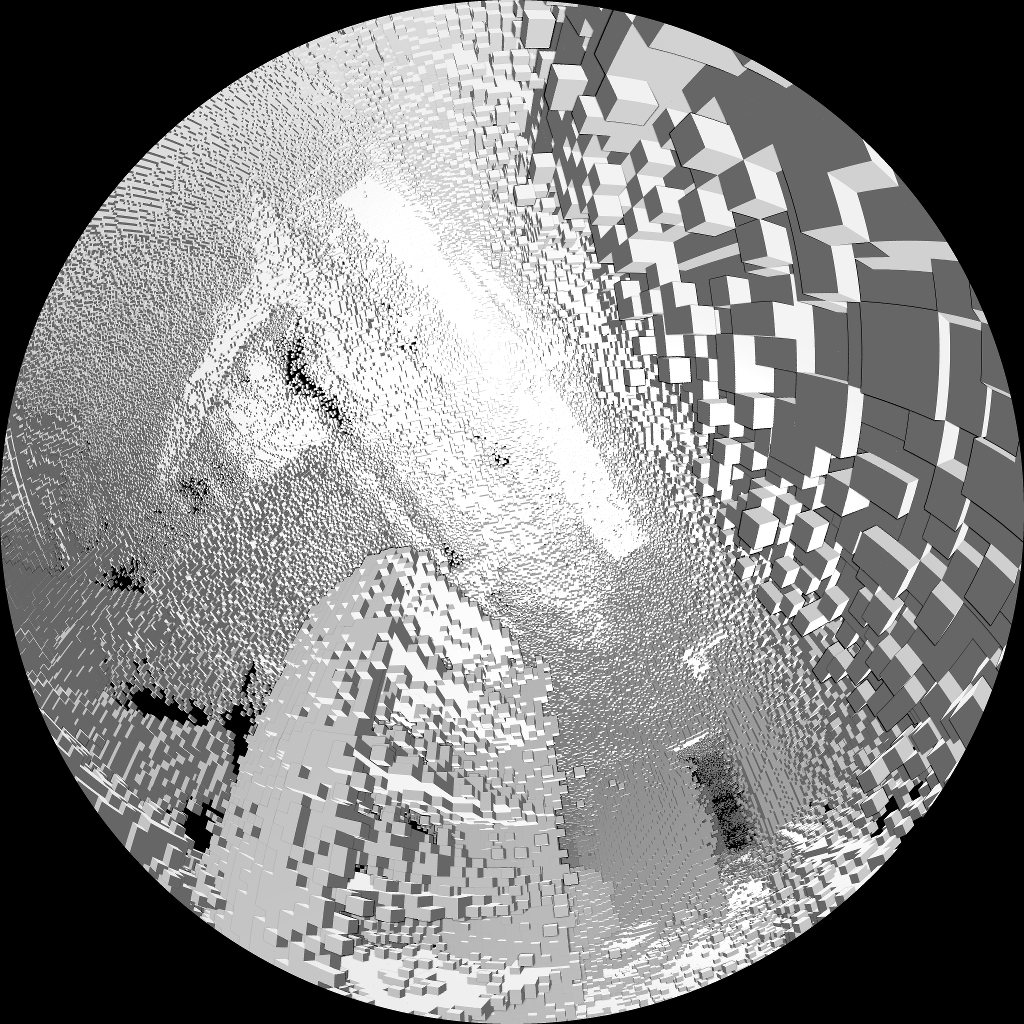
\includegraphics[height=\abImmersiveImageHeight]{figures/fisheye_rendering.png}}
		\label{fig:immersive:fisheye}
	}
	\hfill
	\subfigure[Head-mounted display rendering] {
		\fbox{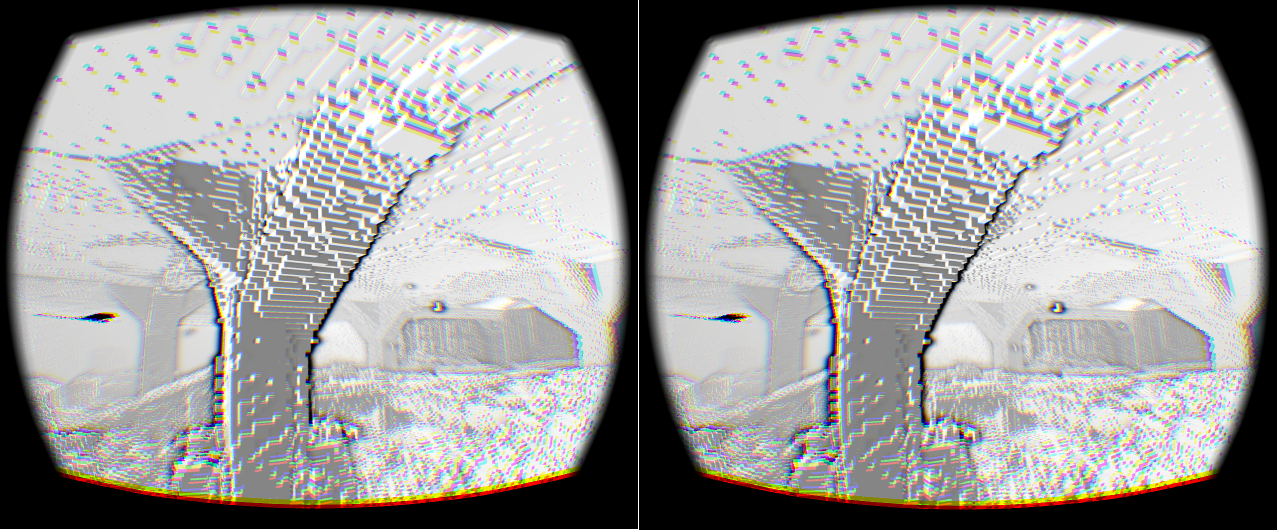
\includegraphics[height=\abImmersiveImageHeight]{figures/hmd_rendering.png}}
		\label{fig:immersive:hmd}
	}
	\caption{Two examples of immersive environments. Rendering the data in a portable dome environment (a) allows many people to analyze the data simultaneously, while head-mounted displays increase the immersion for a single user (b).}
	\label{fig:immersive}
\end{figure*}

\begin{figure*}
	\newcommand{\abResultsImageWidth}{0.3\textwidth}
	\centering
   \subfigure[An ensemble of paths leading away from a construction worker standing on the edge of a pit.] {
       \fbox{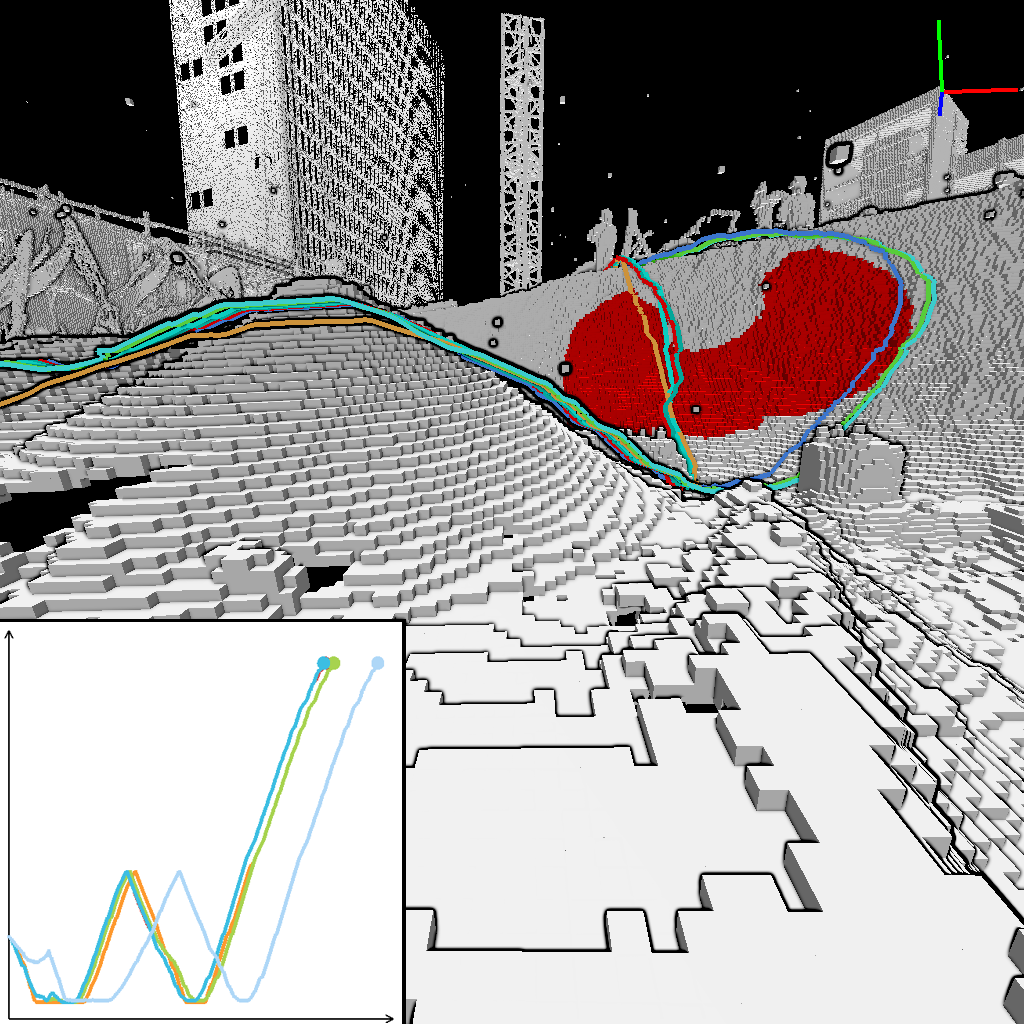
\includegraphics[width=\abResultsImageWidth]{figures/tower-case-path.png}}
    \label{fig:overview:case:tower}
    }
    \hfill{}
    \subfigure[The Bremen rescue arena, which is used to test the autonomy of search \& rescue robots.] {
        \fbox{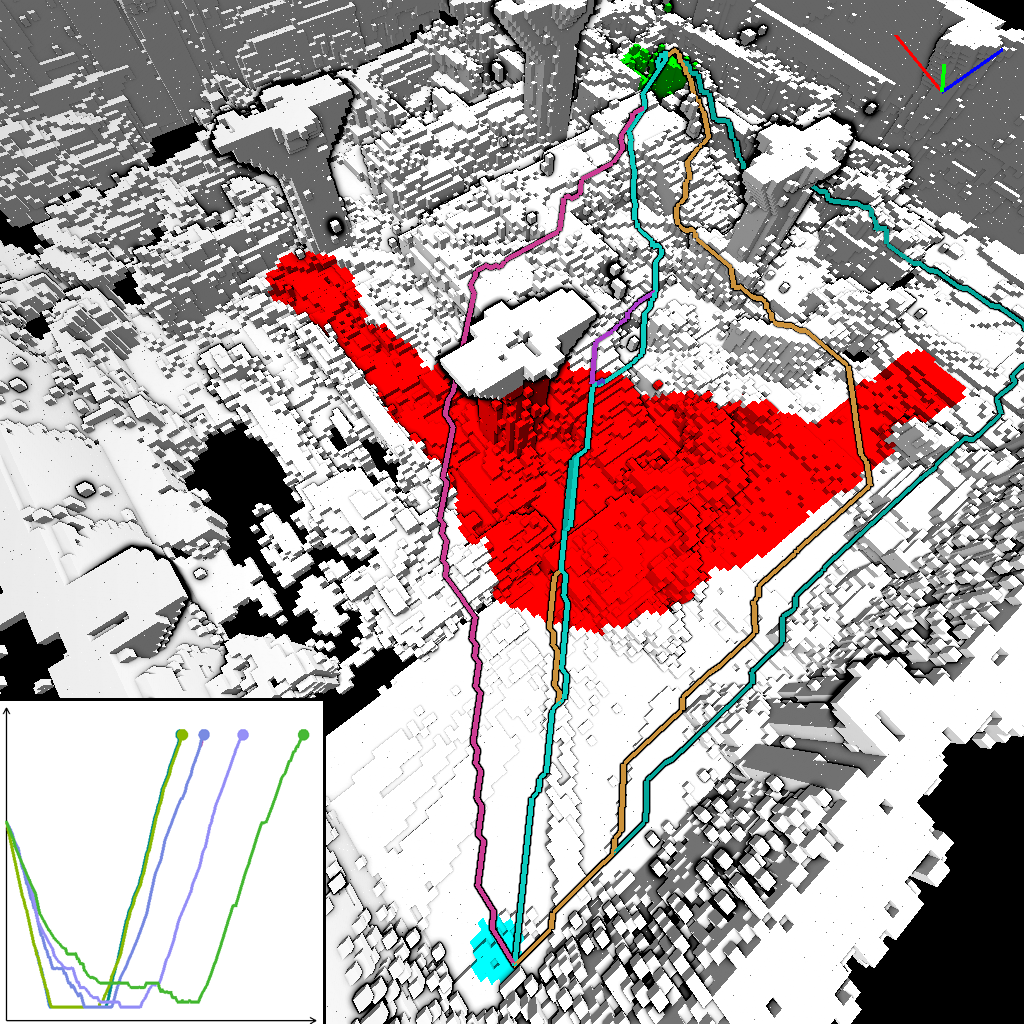
\includegraphics[width=\abResultsImageWidth]{figures/rescue-case-path.png}}
        \label{fig:overview:case:arena}
   }
   \hfill{}
   \subfigure[Three classes of paths in the Tokohu application case at an intermediate step.]{
        \fbox{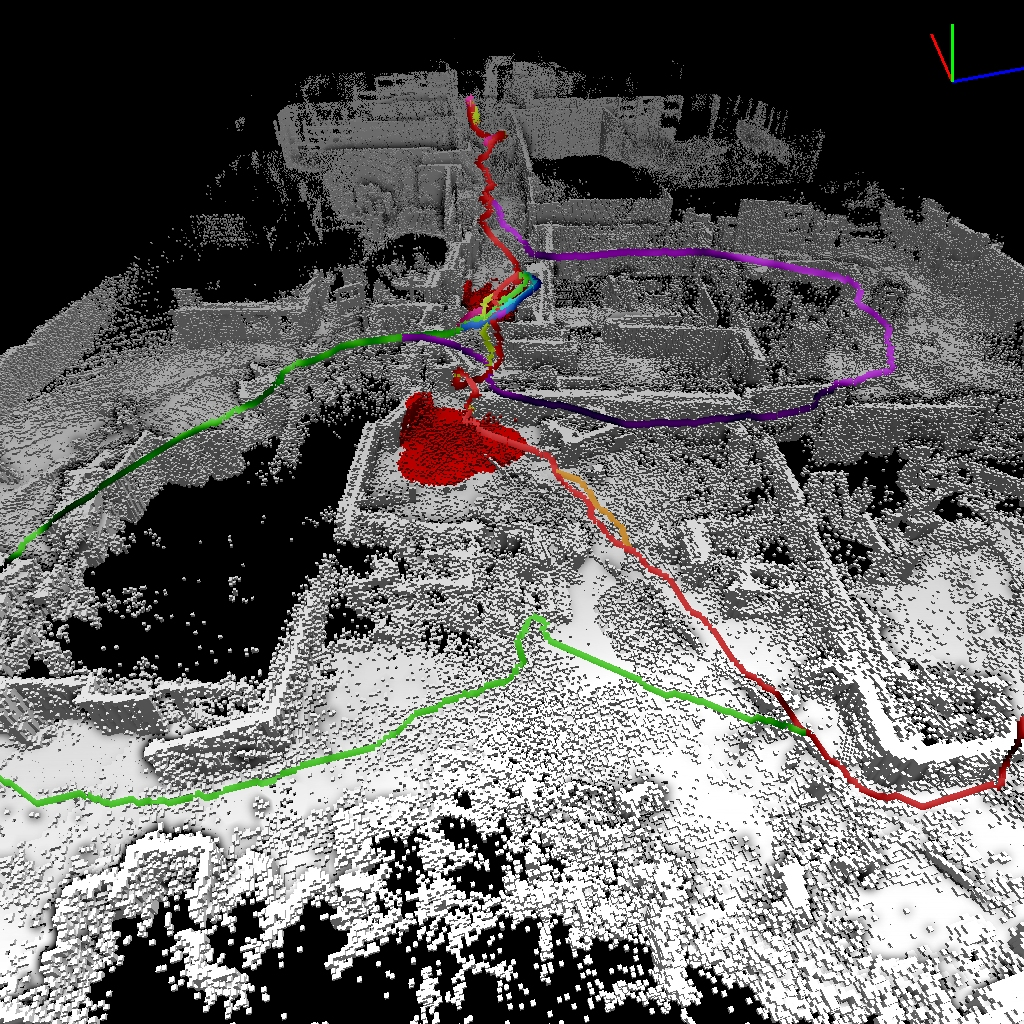
\includegraphics[width=\abResultsImageWidth]{figures/fig-analysis-rendering.jpg}}
        \label{fig:overview:analysis:paths}
   }
   \caption{The rendering component used in the application case (a) and test cases (b) and (c). The filtered paths are shown in the rendering to provide an increased spatial awareness. Different weights for hazards lead to distinct optimal paths to the POI.}
\end{figure*}

\begin{figure*}
	\newcommand{\abImageEnhancementHeight}{0.25\linewidth}
	\centering
	\subfigure[Projective texturing applied to the Bremen Rescue Arena case with a handheld and manually positioned image] {
		\fbox{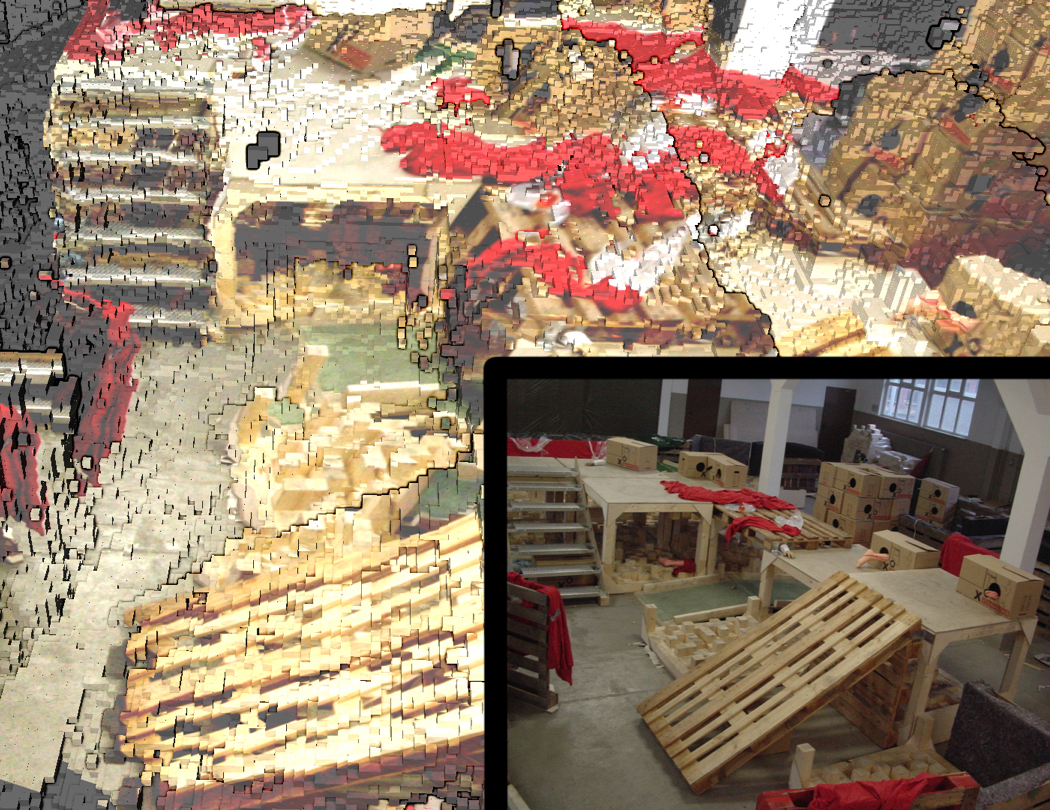
\includegraphics[height=\abImageEnhancementHeight]{figures/projective_texturing.jpg}}
		\label{fig:imageenhancement:texturing}
	}
	\hfill
	\subfigure[The occupancy for each voxel presented by bump mapping. The more occupancy a voxel has, the stronger the bump mapping effect is.] {
		\fbox{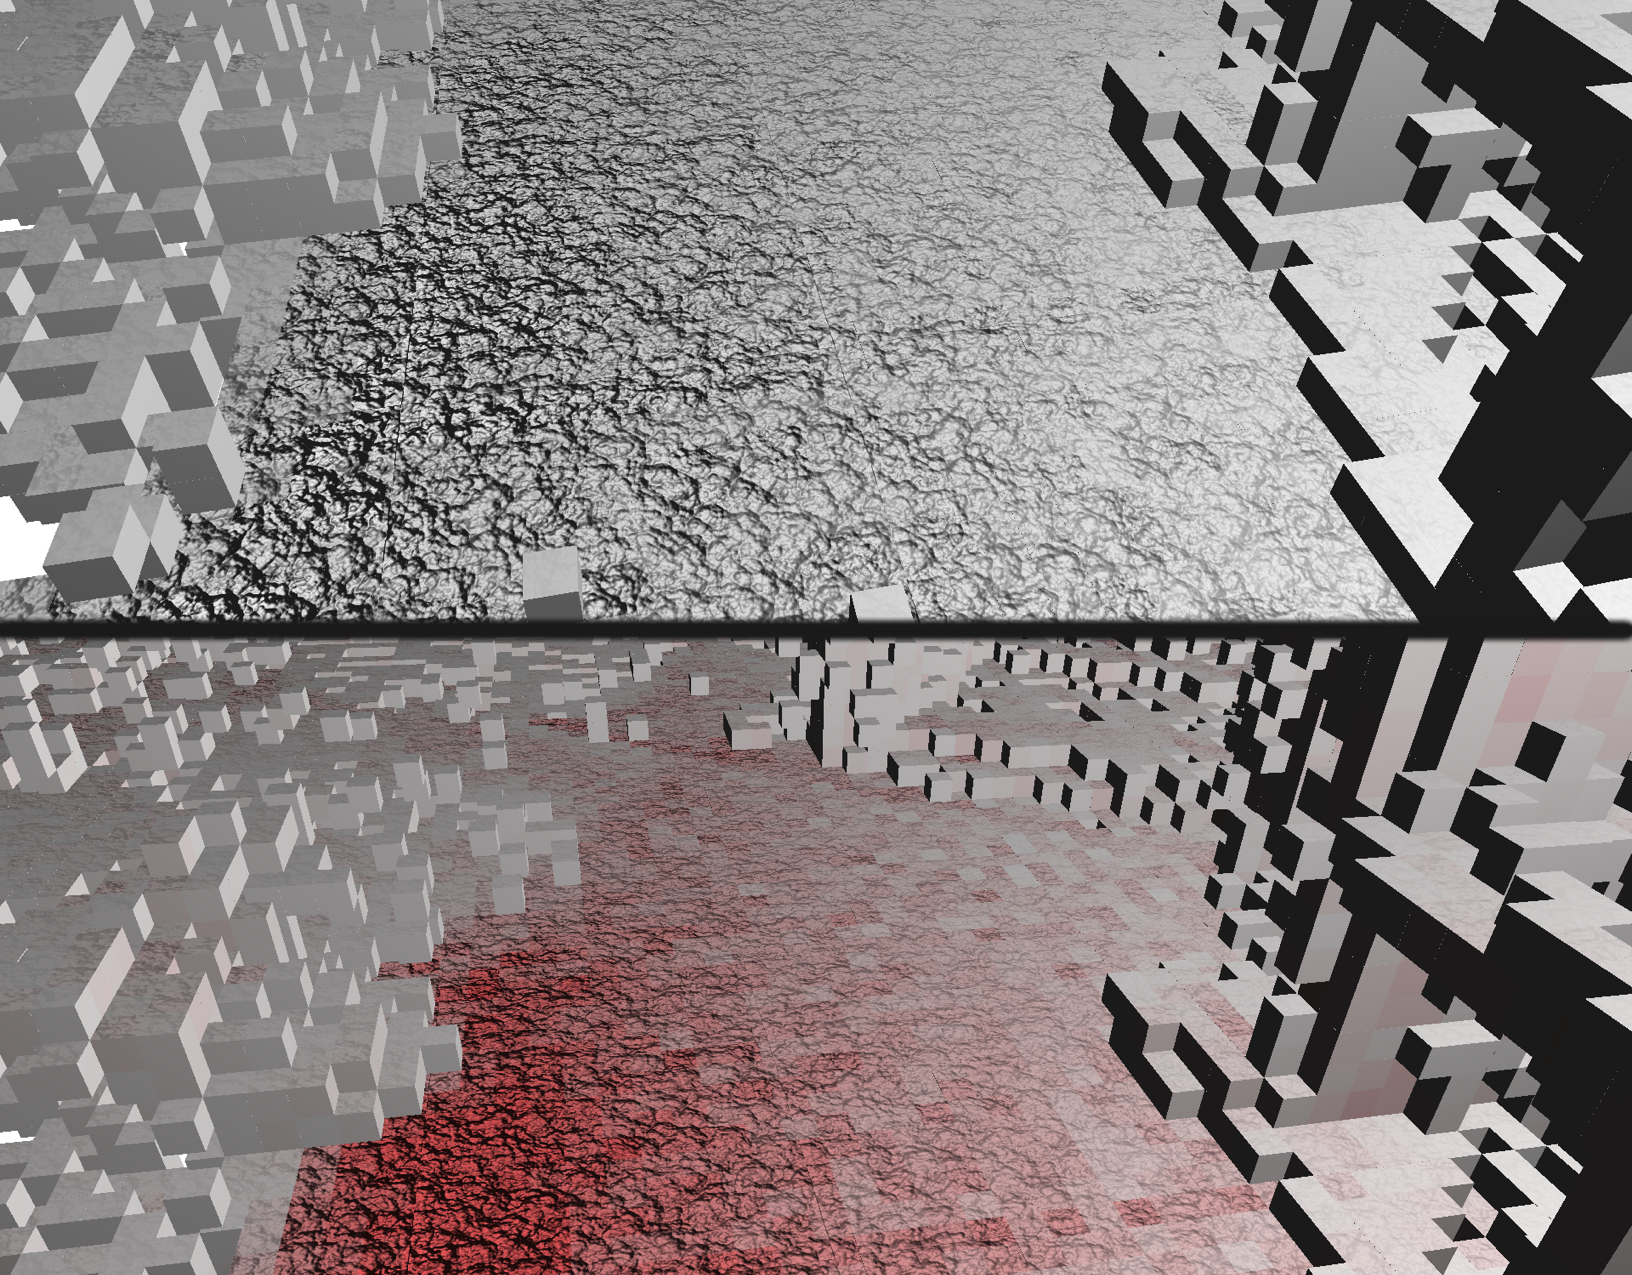
\includegraphics[height=\abImageEnhancementHeight]{figures/occupancy.jpg}}
		\label{fig:imageenhancement:occupancy}
	}
	\hfill
	\subfigure[Attributes derived in the data preprocessing stage. From left: distance to the closest hazard, occupancy, and level of support] {
		\fbox{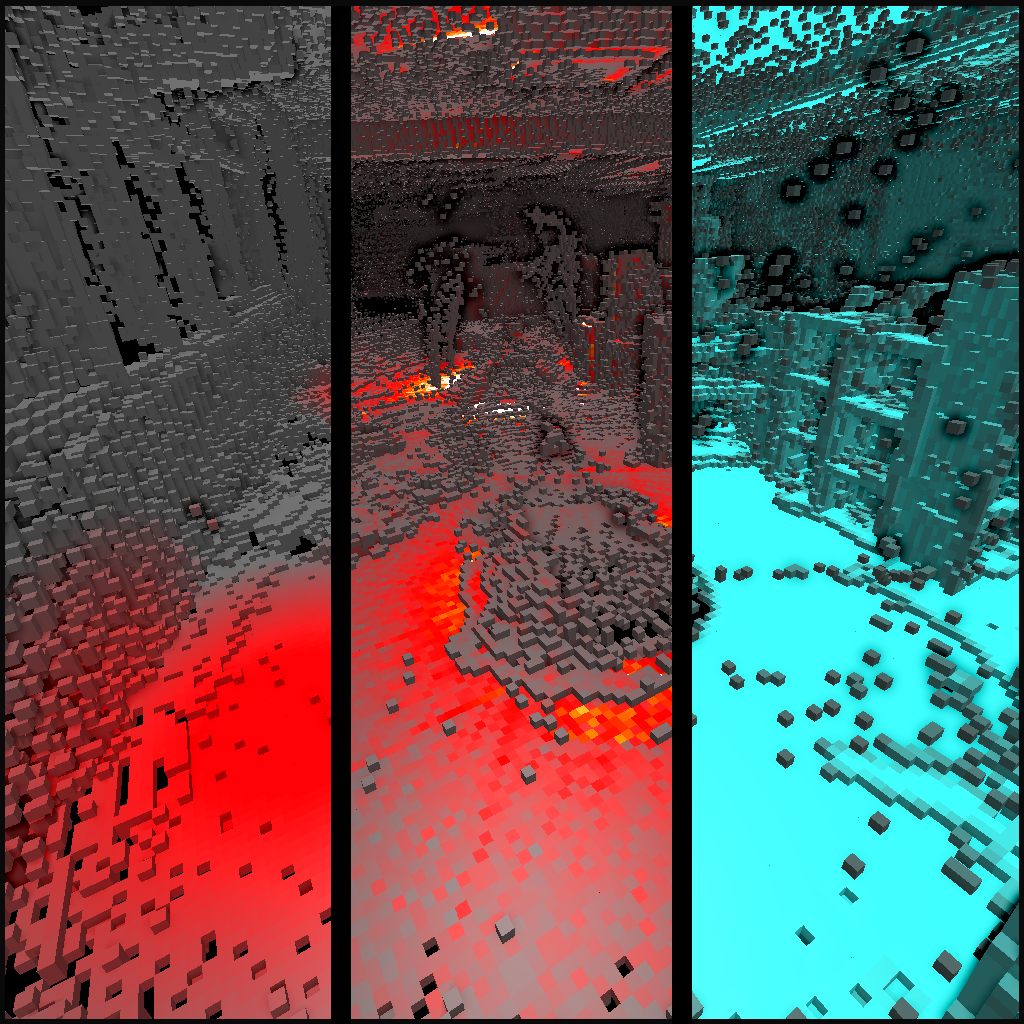
\includegraphics[height=\abImageEnhancementHeight]{figures/fig-overview-fields.png}}
		\label{fig:imageenhancement:colors}
	}
	\caption{The 3D visualization component is enhanced to present the IC with more information about the interior. Projective texturing (a) allows the IC to include images and videos into the environment. Either bump mapping (b) or color coding (c) can be used to show additional information for each voxel.}
	\label{fig:imageenhancement}
\end{figure*}

%%%%%%%%%%%%%%%%%%%%%%%%%%%%%%%%%%%%%%%%%%%%%%%%%%%%%%%%%%%%%%%%%%%%%%%%%%%%%%%%%%%%%%%%%%%
%%%%%%%%%%%%%%%%%%%%%%%%%%%%%%%%%%%%%%%%%%%%%%%%%%%%%%%%%%%%%%%%%%%%%%%%%%%%%%%%%%%%%%%%%%%

\section{Results} \label{sec:results}
Since autonomous robots are not yet used in emergency situations, it is not possible to apply our system to a real-world disaster area. Instead, to illustrate the flexibility of our system, we describe the application to one major application case and two test cases in this section.

\noindent {\bfseries Construction site.} Figure~\ref{fig:overview:case:tower} shows a point cloud acquired at a construction site with a LiDAR scanner being inside an excavation pit. The original dataset consisting of $50$ million points was resampled to $3.5$ million voxels with a voxel size of 5\,cm in 3 minutes 30 seconds on a 3\,GHz four-core CPU. 

\noindent {\bfseries Rescue arena.} Figure~\ref{fig:overview:case:arena} shows an ensemble of paths through the Bremen rescue arena~\cite{varsadan08}, a testing arena built specifically for search \& rescue scenarios. The original point cloud consists of $28$ million points, reduced to $5.3$ million points with 4\,cm resolution.

\subsection{Tohoku Application Case} \label{sec:results:applicationcase}
%\begin{figure}[b]
%    \vspace{-0.5cm}
%    \centering
%    \subfigure[\emph{Standard Deviation of Support} in relation to the \emph{Path Length}] {
%        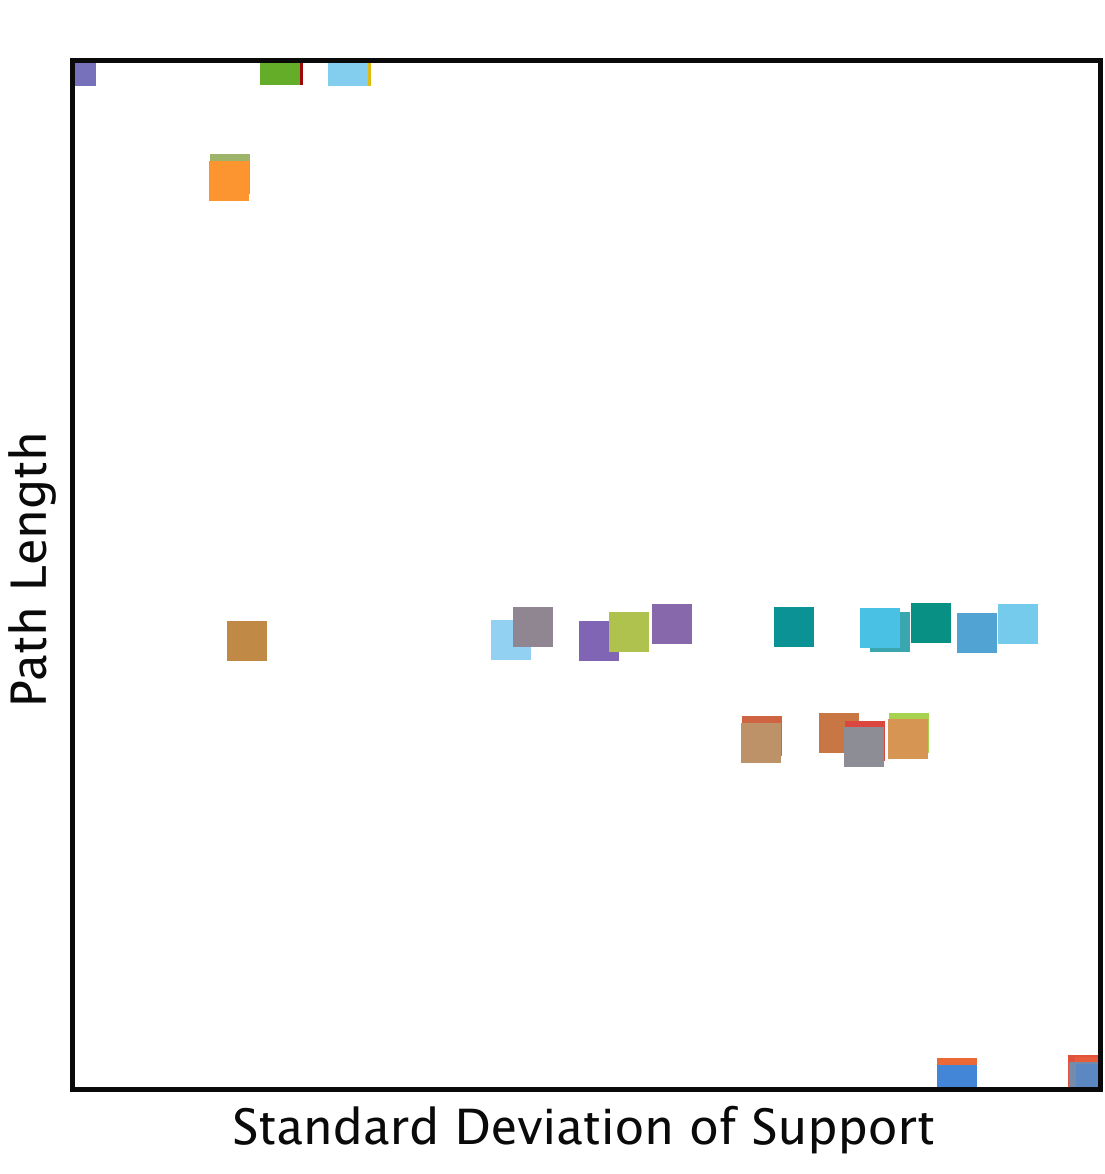
\includegraphics[width=0.3\columnwidth]{figures/pathlength-stddevsupport.png}
%        \label{fig:overview:analysis:lengthstddev}
%    }
%    \hspace{0.5cm}
%    \subfigure[\emph{Average Hazard Distance} in relation to the \emph{Path Length}] {
%        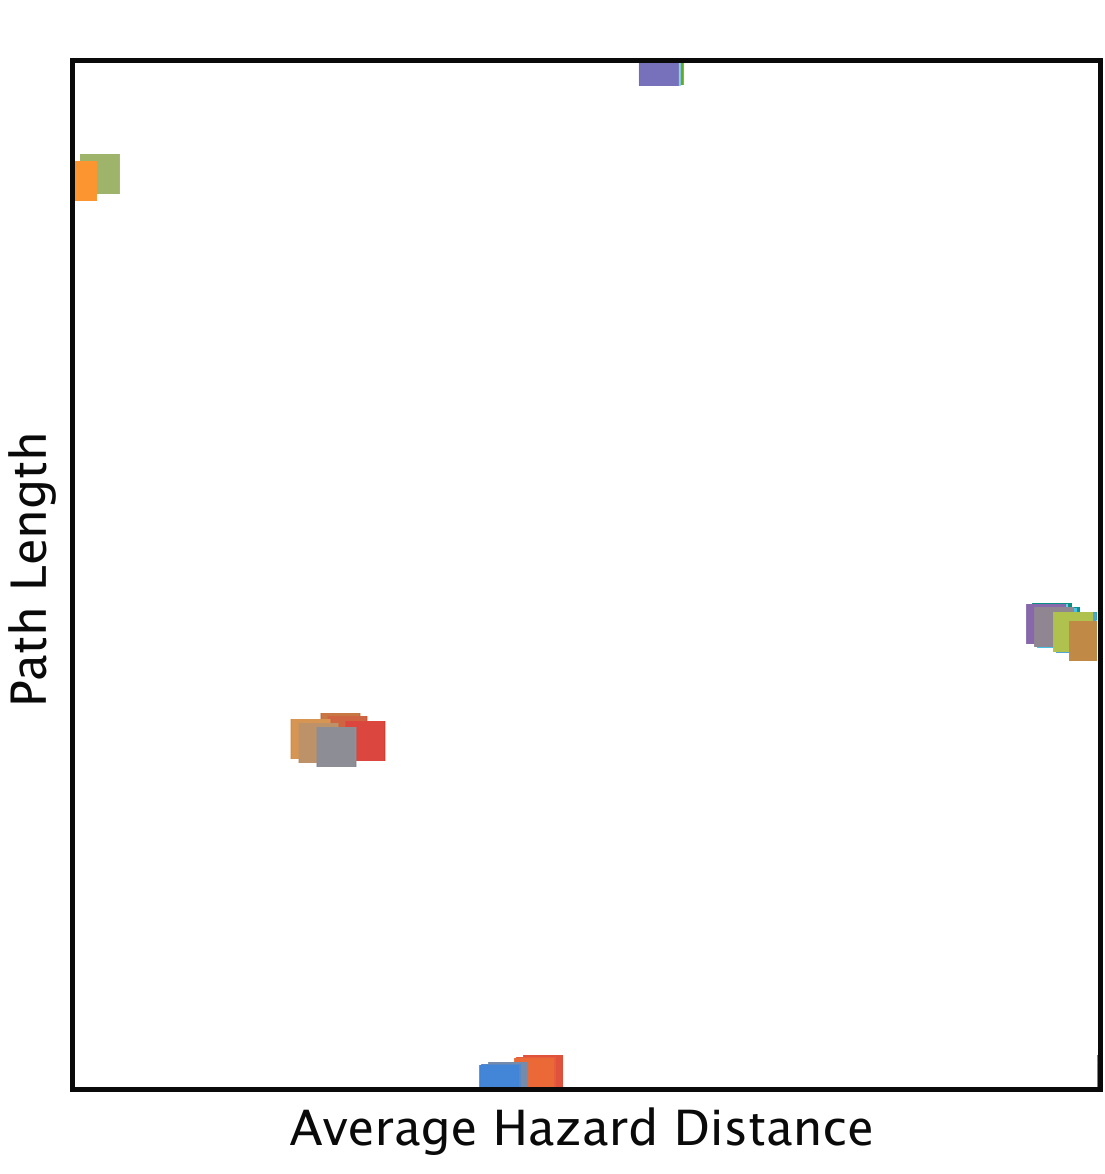
\includegraphics[width=0.3\columnwidth]{figures/pathlength-averagedistance.png}
%        \label{fig:overview:analysis:lengthavg}
%    }
%    \caption{Two zoom-ins of the Scatterplot Matrix (Figure~\ref{fig:overview:analysis:scatter}).  (a) \emph{Standard Deviation of Support} and (n) \emph{Average Hazard Distance} in relation to the \emph{Path Length}.}
%\end{figure}

The major use case is based on three scans from a collapsed building at Tohoku university in the aftermath of the 2011 earthquake in Japan. As there had been partial collapses in the office building, it proved to be a valid and useful simulated real-world application case. The resulting dataset has been acquired with latest state-of-the-art equipment and consists of $26$ million sampling points~\cite{journals/jfr/NagataniKOOYTNYKFK13}, which we resampled to a voxel grid of $4$ million voxels with a voxel size of 3\,cm. Figure~\ref{fig:teaser:1} shows a closeup rendering of the data set with level of detail is sufficient for detailed inspection. Using the same CPU as above and a GeForce GTX 580 graphics card, we achieved average frame rates of about 30\,fps with our system.

No hazards in the building were detected by the robots as this was not part of their mission profile. The task for this application case was as follows: the IC needed to find the shortest path between the entry and the POI. While traversing the path, a rescuer would detect two hazard clouds (red highlights) and the system must be able to react to this change.

Figure~\ref{fig:overview:analysis:paths} shows a subset of computed paths after the second hazard has been discovered. There is one class of paths (purple) that evades the first hazard and another class (green) that evades the second hazard. Figure~\ref{fig:sampling:tohoku} shows the result of the adaptive sampling for the hazard-overhead subspace showing only the unique paths. The parallel coordinates plot (Figure~\ref{fig:overview:analysis:pcp}) makes it possible to detect a path that belongs to both classes with a maximum in the \emph{Minimal Hazard Distance}, while having a long \emph{Path Length}. The scatterplot showing the relationship between \emph{Path Length} and \emph{Standard Deviation of Support} indicates that the shorter paths tend to pass through more unstable areas (see Figure~\ref{fig:overview:analysis:scatter}).

\begin{figure}
	\newcommand{\abImageComparisonWidth}{0.4\linewidth}
	\centering
		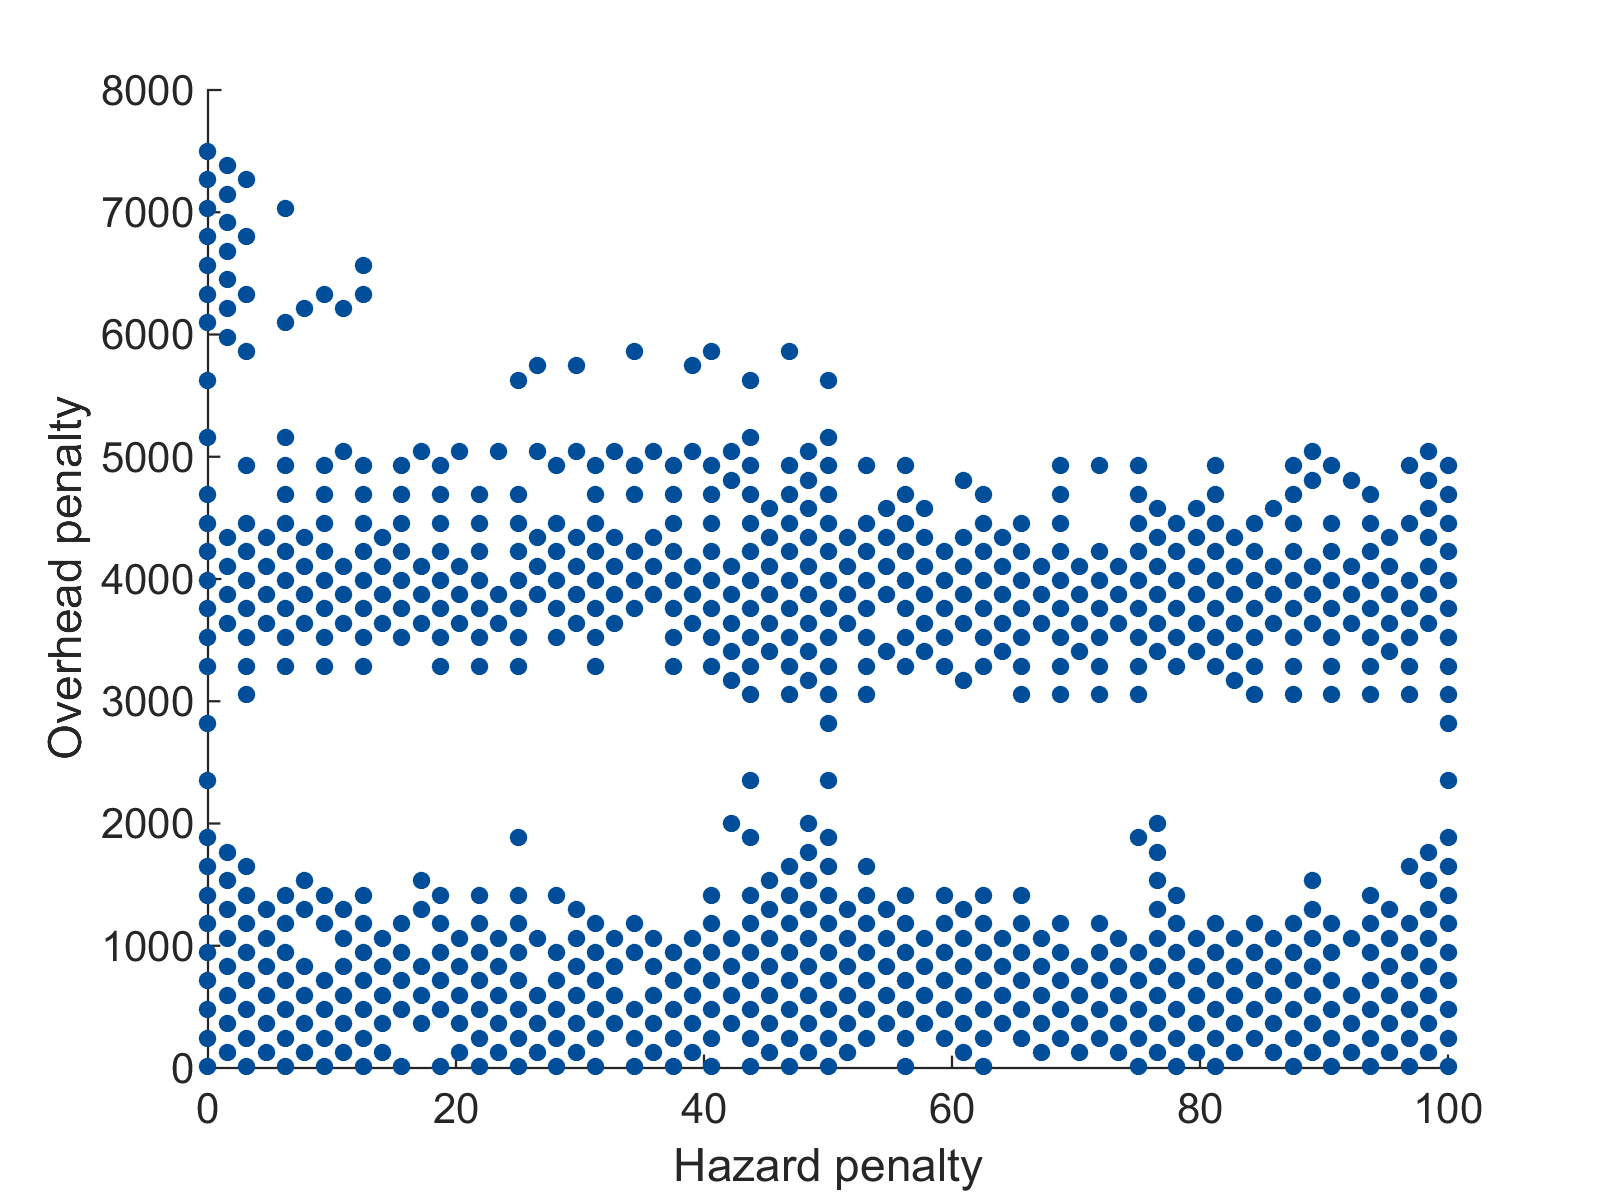
\includegraphics[width=\abImageComparisonWidth]{figures/adaptive_sampling_tohoku.png}
	\caption{The hazard-overhead parameter space for the Tohoku application case showing all the unique paths through the dataset.}
	\label{fig:sampling:tohoku}
\end{figure}

%%%%%%%%%%%%%%%%%%%%%%%%%%%%%%%%%%%%%%%%%%%%%%%%%%%%%%%%%%%%%%%%%%%%%%%%%%%%%%%%%%%%%%%%%%%
%%%%%%%%%%%%%%%%%%%%%%%%%%%%%%%%%%%%%%%%%%%%%%%%%%%%%%%%%%%%%%%%%%%%%%%%%%%%%%%%%%%%%%%%%%%

\section{Evaluation} \label{sec:evaluation}
We performed an evaluation of our system with nine external experts working in the field of Urban Search \& Rescue. Of these experts, five (A--E) are emergency responders, three (F--H) are researchers, and one (J) is a consultant for a national technical relief agency. As the goal of the study was to include as many international experts as possible, and being aware of their time constraints, we decided to create videos and images of our system for the application case and created an interactive webpage rather than requiring training for hands-on use of our system. 7 of 9 experts finished the evaluation and provided answers to all questions. In the analysis, we consider the partial responses for the cases where an answer was provided. The full evaluation and replies are available in the supplemental material. Here, we will discuss important positive and negative answers by the experts. The replies to these questions are on a 5-point Likert scale.

The feedback is grouped into four categories; first, questions letting the experts assess their own knowledge about the component. With these questions, we can estimate whether the experts have prior knowledge and how intuitive the component is. The replies to these questions are on a 5-point Likert scale. The second category are factual checks that have a correct answer. These are used to test if the experts' self-assessment is accurate. The third type of questions are open-ended and allow us insight into the experts' thinking process. Usually, these questions do not have a best answer, but require a trade-off and domain knowledge. The fourth category asks for general comments about a component. The full evaluation and replies are available in the supplemental material. Here, we will discuss important positive and negative answers. 

\noindent \textbf{3D Representation} This component evaluates the general usefulness of the 3D rendering. A video as well as images similar to Figures~\ref{fig:teaser:1},~\ref{fig:teaser:2}, and~\ref{fig:overview:analysis:paths} were provided. We asked to rate the degree of immersion (average: 2.94, $\sigma$: 0.95), the level of knowledge the experts had acquired (average: 2.5, $\sigma$: 0.79), and if the 3D rendering was useful in general (average: 4.14 $\sigma$: 1.20). To test the level of immersion and knowledge of the scene, we asked the experts to describe the room shown in the images, which all performed successfully, leading us to believe that the experts underestimated the knowledge they gained from the 3D rendering. An outlier in the responses was F, who reported 1 for the knowledge and 5 for the usefulness, but described the room correctly. We assume the answers are related to his comment, asking us to ``improve [our] registration algorithm''. \\
%
\textbf{Path Representation} This component tests the usefulness of embedding the paths into the 3D rendering. It shows three images depicting a similar situation as Figure~\ref{fig:teaser:2} with three paths each. We asked the experts which of the paths they would choose and all but two chose the paths that evaded the hazards. A second question was asked to compare the lengths of the shortest and the longest path. While the correct answer was 1.54$\times$, the experts stated an average of 2.56$\times$. This means that, while the experts are capable of estimating the length, they overestimate path distances, making it necessary to provide accurate information in the PP and PCP.\\
%
\noindent \textbf{Evacuation Path Walkthrough} In this component, we evaluated the combined effects of the first two components. We generated two camera paths from the longest path in component 2; one path moving from the \emph{Start} to the \emph{POI} and a second moving opposite. We asked for the usefulness (average: 3.125, $\sigma$: 1.25) and the self-assessed knowledge (average: 2.75, $\sigma$: 0.89) for both paths. \\
%
\textbf{Profile Plot} To evaluate the PP, we provided a reduced plot containing only the orange, green, and yellow paths from Figure~\ref{fig:overview:analysis:profile}. We asked the experts to assess their understanding of the plot (average: 3.5 $\sigma$: 1.30) and its usefulness (average: 3.71 $\sigma$: 1.11). We asked the experts to relate the two longest paths to each other; all eight experts providing answers arrived at the correct conclusion that the orange path is shorter, but crosses the hazard area once. \\
%
\textbf{Parallel Coordinates Plot} The level of self-assessed understanding is lower than the PP (average: 1.66 vs. 3.5, $\sigma$: 0.52 vs. 1.30 ) which can be attributed to the fact the experts might be more familiar with line plots than PCPs. Despite their unfamiliarity, all five experts providing feedback answered identified the shortest and the safest path correctly. This, and the average rated usefulness of 2.14 ($\sigma$: 0.90),  agrees with previous research that a dissociation between preference and performance is common in interface design~\cite{andre1995users}. In the following open questions, the experts favored safe, long paths over shorter, more dangerous paths while not paying much attention to the available support. This confirmed our previous discussion about the ordering of attributes in the PCP.\\
%
\textbf{Scatterplot Matrix} For this representation, the very low level of self-assessed knowledge (average: 1.16, $\sigma$: 0.41) and usefulness (average: 1.28, $\sigma$: 0.49) is, just as the PCP, probably due to the fact that few, if any, experts have worked with SPLOMs before. Only J provided replies to the questions asking for the shortest and the most stable path with regard to the hazard distance, and provided the correct answer. A comment from E summarizes the result for the SPLOM component: ``[this] is more information than I would want to interpret during a SAR mission''. A SPLOM can have a beneficial impact to multivariate analysis~\cite{6064985}, but given the experts' reluctance, we make the SPLOM optional instead.\\
%
\noindent \textbf{Miscellaneous} For the last part, we asked if it is ``helpful to display the paths and [if it] provides additional information'', to which most experts (C, D, E, F, and J) agreed. D noted that the GUI should be more ``user-friendly and understandable'' and J said that ``not detected hazards like structural integrity get visible by the density of scan points''. To the question if they ``[would] like to use [the] system in addition, or as a replacement, to [their] current tools'', B, C, E, F, and J were positive to using our system in addition to their current tools rather than as a replacement. C would like to use it after a ``period of experimentation'', while J sees the system as ``an addition which is warmly welcome''. The only negative comment was from D, who regards the system as too complicated. J suggested a collaboration, saying that the system needs to be more intuitive to allow rescuers, who do not work with SAR operations regularly, to use its full potential.

In conclusion, we received valuable feedback from the experts and we can see that most experts liked the system and would like to use it as a decision-support tool alongside their current applications. With the exception of the SPLOM, the majority of experts were able to retrieve important data from our system and use it for their decision-making.

%%%%%%%%%%%%%%%%%%%%%%%%%%%%%%%%%%%%%%%%%%%%%%%%%%%%%%%%%%%%%%%%%%%%%%%%%%%%%%%%%%%%%%%%%%%
%%%%%%%%%%%%%%%%%%%%%%%%%%%%%%%%%%%%%%%%%%%%%%%%%%%%%%%%%%%%%%%%%%%%%%%%%%%%%%%%%%%%%%%%%%%

\section{Conclusions and Future Work} \label{sec:conclusion}
We presented a visualization system that optimizes the workflow of the IC when dealing with SAR missions. We designed a linked, multiple-view system that computes and analyzes an ensemble of rescue paths. The resulting information is visualized for the IC, who selects a path that is an optimal trade-off according to his experience and knowledge. To investigate the usefulness of the proposed system we have conducted a study with expert users. The resulting feedback makes us confident that the proposed system has the potential to improve future search \& rescue missions.

For future work, we would like to perform a thorough in-use evaluation workshop with rescue experts accompanying a simulated rescue scenario. This will provide us with valuable direct feedback to improve usability of the system. This includes researching methods on how to familiarize the SAR experts with the PCP and the SPLOM method and on the effectivity of using a head-mounted display to inspect the rendering.

%For future work, we like to perform a thorough in-use evaluation workshop with domain experts accompanying a real-world rescue scenario. This will provide us with valuable direct feedback to improve usability of the system. This includes researching methods on how to familiarize the SAR experts with the PCP and the SPLOM method. Furthermore, we plan to investigate the applicability of adaptive and stochastic sampling, like Monte-Carlo methods, on the high-dimensional parameter space for path computation. In addition, we will investigate the possibility of integrating video footage into the 3D point cloud rendering~\cite{1453517}.

%%%%%%%%%%%%%%%%%%%%%%%%%%%%%%%%%%%%%%%%%%%%%%%%%%%%%%%%%%%%%%%%%%%%%%%%%%%%%%%%%%%%%%%%%%%
%%%%%%%%%%%%%%%%%%%%%%%%%%%%%%%%%%%%%%%%%%%%%%%%%%%%%%%%%%%%%%%%%%%%%%%%%%%%%%%%%%%%%%%%%%%

\section*{Acknowledgments}
We like to thank the IRIDeS, the CREATE, and the IRS institutes for retrieving the Tohoku university scans. This work was partly supported by grants from the Excellence Center at Link\"oping and Lund in Information Technology (ELLIIT) and the Swedish e-Science Research Centre (SeRC), as well as VR grant 2011-4113. We thank the external experts for taking part in the evaluation as well as the anonymous reviewers providing helpful feedback. Special thanks goes to Joel Kronander for many fruitful discussions about adaptive sampling methods.

%\newpage 
%\bibliographystyle{eg-alpha-doi}
\bibliographystyle{eg-alpha}
%%use following if all content of bibtex file should be shown
%\nocite{*}
\bibliography{bibliography}

\end{document}
